%%%%%%%%%%%%%%%%%%%% author.tex %%%%%%%%%%%%%%%%%%%%%%%%%%%%%%%%%%%
%
% sample root file for your "contribution" to a contributed volume
%
% Use this file as a template for your own input.
%
%%%%%%%%%%%%%%%% Springer %%%%%%%%%%%%%%%%%%%%%%%%%%%%%%%%%%


% RECOMMENDED %%%%%%%%%%%%%%%%%%%%%%%%%%%%%%%%%%%%%%%%%%%%%%%%%%%
\documentclass[graybox]{svmult}

% choose options for [] as required from the list
% in the Reference Guide

\usepackage{type1cm}        % activate if the above 3 fonts are
                            % not available on your system
%
\usepackage{makeidx}         % allows index generation
\usepackage{graphicx}        % standard LaTeX graphics tool
                             % when including figure files
\usepackage{multicol}        % used for the two-column index
\usepackage[bottom]{footmisc}% places footnotes at page bottom


\usepackage{newtxtext}       % 
\usepackage[varvw]{newtxmath}       % selects Times Roman as basic font




\usepackage{comment}
\usepackage{graphicx}
\usepackage{tikz}
\usepackage{tikz-3dplot}
\usepackage{caption}
\usepackage{subcaption}
%\usepackage{indentfirst}
\usepackage{float}
\usepackage{algpseudocode}
\usepackage{algorithm}
%\usepackage{braket}
\usepackage{commath}
\usepackage{url}
\usetikzlibrary{intersections, calc, math}


\algnewcommand\algorithmicforeach{\textbf{for each}}
\algdef{S}[FOR]{ForEach}[1]{\algorithmicforeach\ #1\ \algorithmicdo}

%\usepackage{svg}

%\usepackage{carshapes}
\usetikzlibrary{angles,quotes}

\usetikzlibrary{calc,arrows.meta,positioning,backgrounds}

%\usepackage[margin=15mm]{geometry}
\usepackage{geometry}
\usepackage{bm}

\usepgfmodule{nonlineartransformations}
\makeatletter
\def\tikz@scan@transform@one@point#1{%
  \tikz@scan@one@point\pgf@process#1%
  \pgf@pos@transform{\pgf@x}{\pgf@y}}
\tikzset{%
  grid source opposite corners/.code args={#1and#2}{%
   \pgfextract@process\tikz@transform@source@southwest{%
     \tikz@scan@transform@one@point{#1}}%
   \pgfextract@process\tikz@transform@source@northeast{%
     \tikz@scan@transform@one@point{#2}}%
  },
  grid target corners/.code args={#1--#2--#3--#4}{%
   \pgfextract@process\tikz@transform@target@southwest{%
     \tikz@scan@transform@one@point{#1}}%
   \pgfextract@process\tikz@transform@target@southeast{%
     \tikz@scan@transform@one@point{#2}}%
   \pgfextract@process\tikz@transform@target@northeast{%
     \tikz@scan@transform@one@point{#3}}%
   \pgfextract@process\tikz@transform@target@northwest{%
     \tikz@scan@transform@one@point{#4}}%
  }
}

\def\tikzgridtransform{%
  \pgfextract@process\tikz@current@point{}%
  \pgf@process{%
    \pgfpointdiff{\tikz@transform@source@southwest}%
      {\tikz@transform@source@northeast}%
  }%
  \pgf@xc=\pgf@x\pgf@yc=\pgf@y%
  \pgf@process{%
    \pgfpointdiff{\tikz@transform@source@southwest}{\tikz@current@point}%
  }%
  \pgfmathparse{\pgf@x/\pgf@xc}\let\tikz@tx=\pgfmathresult%
  \pgfmathparse{\pgf@y/\pgf@yc}\let\tikz@ty=\pgfmathresult%
  %
  \pgfpointlineattime{\tikz@ty}{%
    \pgfpointlineattime{\tikz@tx}{\tikz@transform@target@southwest}%
      {\tikz@transform@target@southeast}}{%
    \pgfpointlineattime{\tikz@tx}{\tikz@transform@target@northwest}%
      {\tikz@transform@target@northeast}}%
}

\newcommand{\savedx}{0}
\newcommand{\savedy}{0}
\newcommand{\savedz}{0}

\newcommand{\somedrawing}%
{   \coordinate (a) at (-2,-2,-2);
    \coordinate (b) at (-2,-2,2);
    \coordinate (c) at (-2,2,-2);
    \coordinate (d) at (-2,2,2);
    \coordinate (e) at (2,-2,-2);
    \coordinate (f) at (2,-2,2);
    \coordinate (g) at (2,2,-2);
    \coordinate (h) at (2,2,2);
    \draw (a)--(b) (a)--(c) (a)--(e) (b)--(d) (b)--(f) (c)--(d) (c)--(g) (d)--(h) (e)--(f) (e)--(g) (f)--(h) (g)--(h);
    \fill (a) circle (0.1cm);
    \fill (d) ++(0.1cm,0.1cm) rectangle ++(-0.2cm,-0.2cm);
}

\newcommand{\rotateRPY}[4][0/0/0]% point to be saved to \savedxyz, roll, pitch, yaw
{   \pgfmathsetmacro{\rollangle}{#2}
    \pgfmathsetmacro{\pitchangle}{#3}
    \pgfmathsetmacro{\yawangle}{#4}

    % to what vector is the x unit vector transformed, and which 2D vector is this?
    \pgfmathsetmacro{\newxx}{cos(\yawangle)*cos(\pitchangle)}% a
    \pgfmathsetmacro{\newxy}{sin(\yawangle)*cos(\pitchangle)}% d
    \pgfmathsetmacro{\newxz}{-sin(\pitchangle)}% g
    \path (\newxx,\newxy,\newxz);
    \pgfgetlastxy{\nxx}{\nxy};

    % to what vector is the y unit vector transformed, and which 2D vector is this?
    \pgfmathsetmacro{\newyx}{cos(\yawangle)*sin(\pitchangle)*sin(\rollangle)-sin(\yawangle)*cos(\rollangle)}% b
    \pgfmathsetmacro{\newyy}{sin(\yawangle)*sin(\pitchangle)*sin(\rollangle)+ cos(\yawangle)*cos(\rollangle)}% e
    \pgfmathsetmacro{\newyz}{cos(\pitchangle)*sin(\rollangle)}% h
    \path (\newyx,\newyy,\newyz);
    \pgfgetlastxy{\nyx}{\nyy};

    % to what vector is the z unit vector transformed, and which 2D vector is this?
    \pgfmathsetmacro{\newzx}{cos(\yawangle)*sin(\pitchangle)*cos(\rollangle)+ sin(\yawangle)*sin(\rollangle)}
    \pgfmathsetmacro{\newzy}{sin(\yawangle)*sin(\pitchangle)*cos(\rollangle)-cos(\yawangle)*sin(\rollangle)}
    \pgfmathsetmacro{\newzz}{cos(\pitchangle)*cos(\rollangle)}
    \path (\newzx,\newzy,\newzz);
    \pgfgetlastxy{\nzx}{\nzy};

    % transform the point given by #1
    \foreach \x/\y/\z in {#1}
    {   \pgfmathsetmacro{\transformedx}{\x*\newxx+\y*\newyx+\z*\newzx}
        \pgfmathsetmacro{\transformedy}{\x*\newxy+\y*\newyy+\z*\newzy}
        \pgfmathsetmacro{\transformedz}{\x*\newxz+\y*\newyz+\z*\newzz}
        \xdef\savedx{\transformedx}
        \xdef\savedy{\transformedy}
        \xdef\savedz{\transformedz}     
    }
}

\tikzset{RPY/.style={x={(\nxx,\nxy)},y={(\nyx,\nyy)},z={(\nzx,\nzy)}}}

\newcommand{\MarkRightAngle}[4][.3cm]% #1=size (optional), #2-#4 three points: \angle #2#3#4
{\coordinate (tempa) at ($(#3)!#1!(#2)$);
 \coordinate (tempb) at ($(#3)!#1!(#4)$);
 \coordinate (tempc) at ($(tempa)!0.5!(tempb)$);%midpoint
 \draw (tempa) -- ($(#3)!2!(tempc)$) -- (tempb);
} 



% see the list of further useful packages
% in the Reference Guide

\makeindex             % used for the subject index
                       % please use the style svind.ist with
                       % your makeindex program

%%%%%%%%%%%%%%%%%%%%%%%%%%%%%%%%%%%%%%%%%%%%%%%%%%%%%%%%%%%%%%%%%%%%%%%%%%%%%%%%%%%%%%%%%

\begin{document}

\title*{Lifting 2D Object Detection to 3D: \\ 
Geometric Approach in Bird-Eye-View}
% Use \titlerunning{Short Title} for an abbreviated version of
% your contribution title if the original one is too long
\author{Dmitriy Zhuravlev}
% Use \authorrunning{Short Title} for an abbreviated version of
% your contribution title if the original one is too long
\authorrunning{Lifting 2D object detection to 3D in BEV}
\institute{D. Zhuravlev \at Taras Shevchenko National University of Kyiv, \email{dzhuravlev@ukr.net}}
%\and Name of Second Author \at Name, Address of Institute \email{name@email.address}}
%
% Use the package "url.sty" to avoid
% problems with special characters
% used in your e-mail or web address
%
\maketitle

\abstract*{3D object detection is fundamental for computer vision applications.
Although motion is essentially linked with the orientation of the object, the trajectory of the object is not fully utilized in modern 3D object detectors.
This paper proposes a method for object 3D bounding box estimation based on 2D tracking and Inverse Perspective Mapping.
Unlike other solutions utilizing deep learning techniques for orientation estimation, the proposed method uses geometric constraints and object movements.
Which causes the execution speed and errors of 3D localization to remain comparable to a pure 2D tracker.}

\abstract{3D object detection is fundamental for computer vision applications.
Although the motion is essentially linked with the orientation of the object, the trajectory of the object is not fully utilized in modern 3D object detectors.\newline\indent
This paper proposes a method for object 3D bounding box estimation based on 2D tracking and Inverse Perspective Mapping.
Unlike other solutions utilizing deep learning techniques for orientation estimation, the proposed method uses geometric constraints and object movements.
This causes the execution speed and errors of 3D localization to remain comparable to a pure 2D tracker.}

\section{Introduction}
\label{sec:1}
Detecting 3D objects is one of the key components of computer vision. It recovers orientation, position, and the size of an object within a scene.
While developed 2D detection algorithms are capable of processing 
large amounts of data in real-time
\cite{yolo_paper, trafic}, accurately detecting 3D objects remains challenging.

Special equipment-based methods, including LiDAR scanners \cite{lidar} and RGB-D cameras \cite{3d_cam}  provide an approach for 3D direct object reconstruction, but the equipment is quite expensive.

Monocular camera-based methods \cite{3d_geom}, on the contrary, are attractive because of their cheaper cost and more flexible setup. However, the main disadvantage of using a monocular camera is that it only conducts observations in the plane of a two-dimensional image and is unable to directly measure the distance to an object.
That is why it becomes important but still a challenge for cost-effective autonomous tracking and virtual reality. 
%This paper focuses on detecting complete 3D object using only an RGB monocular image.

While the recently developed
2D detection algorithms are capable of detecting and tracking large amounts of data in real time, accurate detection of 3D objects
remains an open problem despite some recent promising findings.
The difference between detecting 2D and 3D objects is significant. Solid shapes have three dimensions, center localization and orientation angles, whereas flat figures are limited by an axis-aligned rectangle with two dimensions. 

The goal of this paper is to effectively infer the 3D bounding box on top of conventional 2D box object detection using the sequence of monocular images.
We introduce the lifting pipeline that can be used with any 2D detection and tracking algorithms providing reliable results.
The main contributions of this paper can be summarized as follows:
\begin{itemize}
   % \item A scheme for 3D localization based on 2D bounding box, object orientation and dimensions
    %\item An approach for possible orientations calculation based on geometric constraints;
    \item a method for object orientation estimation via  2D boxes centers tracking;
    \item a geometric analysis of the relation between detection 2D box, orientation, and object sizes;
 %   \item An approach for possible orientations calculation based on geometric constraints;
 %   \item A method for correction estimated orientation based on geometric constraints;
    \item a scheme for converting 2D tracking to 3D;
   % \item A method for 3D localization via  2D boxes centers tracking.
    \item a design of an end-to-end baseline architecture demonstrating reasonable performance and accuracy.
\end{itemize}


The remainder of this paper is organized as follows. In the next section, the review of popular 3D object detection techniques is given. 
Sect.~\ref{sec:back}  introduces a set of necessary concepts that will be used later in our method from Sect.~\ref{sec:meth}.
The results of real-world testing with a concluding summary are presented in Sect.~\ref{sec:res}.

\section{Related work}
This section discusses the existing methods for 3D localization that intend to recreate the depth information from an RGB image.

Like most of the works related to 3D object detection from a single image, \cite{3d_geom} proposed a method for regression of an observation angle and 3D object sizes from the cropped image patch enclosed by 2D detection box. Using the regressed dimensions and orientations of the 3D box and 2D detection box they try to minimize the re-projection error related to the initial 2D detection box constraints.
Since each side of the 2D detection box can correspond to any of the eight corners of the 3D box, there are $8^4$ configurations.


In the \cite{3d_geom_reduced} the number of plausible configurations is reduced to $64$.
These configurations go through equations to find the vertices of a cuboid and the resulting solutions are ranked by approximation error or intersection over union (IoU) score between the tightest bounding box for the projected vertices of the fitted cuboid and the 2D detection rectangle.

%there are many options from which you need to choose the best, which does not allow using these methods in real-time applications.

To simplify object distance measurement, the Bird's Eye View (BEV) based architecture is proposed in  
\cite{bev_1}. Since all traffic participants are in contact with the ground, the distance can be estimated as detection of points of contact of the vehicle with the road. The proposed method involves two stages: motion cancellation and the detection of position, size,
and orientation using convolutional neural networks. In this work, two types of detectors for rotated boxes prediction on BEV are proposed.
The one-stage detectors have the advantage of fast operating speed because of direct prediction of the bounding box from the feature map grid without refinement.
On the other hand, two-stage detectors predict the position and size of the object more precisely since the network predicts the box proposal and performs refinement in two steps.
However, such defectors operate slower.


\cite{bev_2} extends the previous approach for uncalibrated traffic cameras using dual-view architecture.
In this architecture, both the original view and BEV images are taken as input. The original view feature maps are warped
to BEV and concatenated with BEV feature maps. The dual-view structure enables feature learning before warping, where the object shapes are regular and the
knowledge propagation is easier but it still has the two-stage detectors issues.


In \cite{bev_mod} the idea of learning moving object detection directly in BEV space is explored. 
The architecture based on two-stream RGB and optical flow fusion is proposed for object localization.
However, the lengths of some objects are not captured perfectly and some of the objects are misclassified as false static objects, which shows that there is still room for
improvement.

Moving object detection has received a lot of attention recently, especially in autonomous driving applications. Traffic information can be used as a signal for class-independent detection.
Motion segmentation has been explored in \cite{bev_mod} in order to predict object-moving in BEV using RGB image and optical flow.

All the mentioned methods study 3D object localization using different neural networks which not only get a 2D box but also extract additional information from the image to predict the distance and orientation.
However, geometric constraints of moving objects are not explored enough. 
In this work, we identify real-world scenarios where high reconstruction accuracy is guaranteed via the geometric analysis and apply our algorithm to localize 3D object in real-time.




\section{Background} \label{sec:back}
\subsection{Camera model}

\begin{figure}%[H]
\centering
\tdplotsetmaincoords{-60}{-35}
\begin{tikzpicture}
  [
    tdplot_main_coords,
    >=Stealth,
    my dashed/.style={dashed, thick, ->, shorten >=-15pt, shorten <=-15pt, every node/.append style={font=\footnotesize}},
    my box/.style={thin, gray!70},
    my blue/.style={blue, line cap=round, -{Triangle[width=3*#1]}, line width=#1, shorten >=#1*1.75pt, every node/.append style={fill, circle, inner sep=0pt, minimum size=#1*3.5pt, anchor=center, outer sep=0pt}},
    my label/.append style={midway, font=\scriptsize},
    my vectors/.style={green!50!black, {Stealth[scale=.75]}-{Stealth[scale=.75]}},
    my red/.style={thick, red, line cap=round},
    my grey/.style={gray!70},
    description/.style={draw=gray!70, thick, line cap=round, every node/.style={align=center, font=\scriptsize\sffamily, anchor=north}},
  ]
%   \draw [help lines] (-2,0,0) -- (2,0,0) node[anchor=north west]{$x$} (0,0,0) -- (0,7,0) node[anchor=north east]{$y$} (0,0,0) -- (0,0,2) node[anchor=north]{$z$} (-2,7,0) -- (2,7,0);
  \draw [my grey] (0,4,0) -- (0,7,0) (-2,7,0) -- (2,7,0);
  \coordinate (o) at (0,0,0);
  \path [draw=gray!70, text=gray, fill=gray!20, opacity=0.8, text opacity=1] (-1.5,4,1.75) coordinate (a) -- ++(0,0,-3.5) coordinate (b) -- ++(3,0,0) coordinate (c) -- ++(0,0,3.5) coordinate (d) -- cycle node [pos=.95, above, sloped, anchor=south west] {$z=f$} ;
%   \foreach \i in {a,b,c,d} \node [red, font=\scriptsize] at (\i) {\i};
  \draw [my grey] (-2,0,0) -- (2,0,0) (0,0,0) -- (0,4,0) (0,0,0) -- (0,0,2);
  \draw [thick, ->, every node/.style={font=\footnotesize, inner sep=0pt}] (o) node [anchor=north west] {$O_c$} (o) edge node [pos=1, anchor=north east] {$z_c$} ++(0,1,0) edge node [pos=1, anchor=north] {$y_c$} ++(0,0,1) -- ++(1,0,0) node [anchor=north west] {$x_c$};
  \draw [my box] (o) ++(0,4,-.5) coordinate (p1) -- ++(1,0,0) coordinate (p2) -- ++(0,0,-1.25) coordinate (p3);
  \foreach \i in {0,1,...,4} \draw [my box] (p1) ++(\i*.25,0,0) -- ++(0,0,-.25);
  \foreach \i in {0,1,...,5} \draw [my box] (p2) ++(0,0,-\i*.25) -- ++(-.25,0,0);
  \draw [my box] (p1) ++(0,0,-.25) -- ++(.75,0,0) -- ++(0,0,-1);
  \draw [my dashed, cyan] ($(b)!1/2!(c)$) -- ($(d)!1/2!(a)$) node [below=15pt, anchor=north] {$y$};
  \draw [my dashed, cyan] ($(b)!1/2!(a)$) -- ($(d)!1/2!(c)$) node [above right=17pt, anchor=north west] {$x$};
  \draw [my dashed, green!50!black, <->] (a) node [below=15pt, anchor=north] {$v$} -- (b) -- (c) node [above right=17pt, anchor=north west] {$u$};
  \path [green!50!black, every node/.style={font=\scriptsize, inner sep=0pt}] (p2) node [above right, anchor=south west] {$(u,v)$};
  \path (p2) ++(-.125,0,0) coordinate (q2) ++(0,0,-.125) coordinate (r2);
  \draw [my blue=1] ($(0,4,0)+($(q2)-(p1)$)$) coordinate (s2) -- (r2) node (d1) {};
  \scoped[on background layer]{\draw [my blue=1.75] ($($1.75*($(s2)-(0,4,0)$)$)+(0,7,0)$) -- ++($1.75*($(r2)-(s2)$)$) node (d2) [label={[label distance=-20pt]above:{$p=(x,y,z)$}}] {};}
  \draw [my vectors] (0,4,.1) -- ($(s2)+(0,0,.1)$) node [below, my label, sloped] {$\vec{u}$};
  \draw [my vectors] (-.1,4,0) -- ($(q2)-(s2)+(-.1,4,0)$) node [left, my label] {$\vec{v}$};
  \draw [my red] (o) -- (d1.center);
  \scoped[on background layer]{\draw [my red] (d1.center) -- (d2.center);}
  \path [description] (0,4,0) [out=-95, in=95] to (-.75,4,.25) node {principal\\point} (0,6.5,0) [out=-95, in=95] to (-.75,6.5,.25) node {optical\\axis};
\end{tikzpicture}
\caption{Pinhole camera model}
\label{fig:camera}
\end{figure}


The camera model is a basis for developing a computer vision application. In this article,
the simplest model as shown in Fig.~\ref{fig:camera} with no distortion factor is used to describe the projection of 3D points onto an image plane. % as shown in the Figure~\ref{fig:camera}.\\

Let us describe the correspondences between the camera, world, and picture coordinate systems.
Let $p = (x_w, y_w, z_w)$ be a 3D point in the world coordinate system.
It can be transformed into camera coordinates using the \textbf{extrinsic matrix} which consists of the rotation $\textbf{R} \in \mathbb{SO}(3)$  and translation $\textbf{t} \in \mathbb{R}^3$ between the two coordinate systems.
    $$
     \begin{bmatrix}
	 x_c\\y_c\\z_c		
	 \end{bmatrix}
	 =
	 \textbf{R}
	 \begin{bmatrix}
	 x_w\\y_w\\z_w		
	 \end{bmatrix}
	 + \textbf{t}
	 \label{eq:wc}
$$

The new 3D point in the camera coordinate system is projected onto the image plane using the \textbf{intrinsic matrix} $\textbf{K}$ which consists of internal camera parameters like the focal length, optical center, etc.
$$
\begin{bmatrix}
		u'\\v'\\w'
		\end{bmatrix}=		
		 \textbf{K}
		\begin{bmatrix}
		x_{c}\\y_{c}\\z_{c}
		\end{bmatrix}
    \label{eq:k1}
$$
where $u = \frac{u'}{w'}$, $v = \frac{v'}{w'}$.\\
The overall projection in homogeneous coordinates can be expressed by:
$$ \begin{bmatrix}
		u'\\v'\\w'
		\end{bmatrix}=
		\textbf{K} \left(\textbf{R}
		\begin{bmatrix}
	    x_w\\y_w\\z_w		
	    \end{bmatrix}
		+ \textbf{t} \right)$$. % as shown in  Figure~\ref{fig:camera}.



\subsection{Inverse perspective mapping}
The distance of the object from the camera and the observation angle should be taken into account for reconstruction
the ground plane as if viewed from a camera placed above with its axis exactly vertical.
\textbf{Inverse Perspective Mapping} (IPM) uses the frontal view to produce a \textbf{Bird’s Eye View} (BEV) by removing perspective effects using a homography. The example of the IPM is shown in Fig.~\ref{fig:ipm}.

\begin{figure}%[H]
    \centering
    \begin{subfigure}[t]{0.4\textwidth}
        \centering
            \resizebox{.8\textwidth}{!}{%
            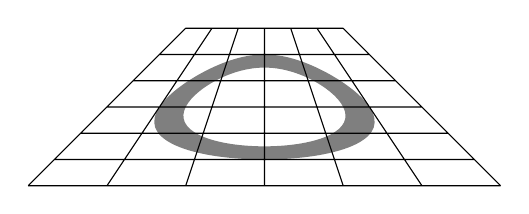
\begin{tikzpicture}
                \begin{scope}[
                grid source opposite corners={(0,0) and (6,6)},
                grid target corners={(1,1) -- (7,1) -- (5,3) -- (3,3)}]
            \pgftransformnonlinear\tikzgridtransform
            \draw (0,0) grid (6,6);
            \fill [even odd rule, opacity=0.5] 
         (3,3) circle [radius=2] circle [radius=1.5];
        \end{scope}
        \end{tikzpicture}
            }
        \caption{Perspective view}
    \end{subfigure}%
    ~ 
    \begin{subfigure}[t]{0.4\textwidth}
        \centering
         \resizebox{.6\textwidth}{!}{%
                     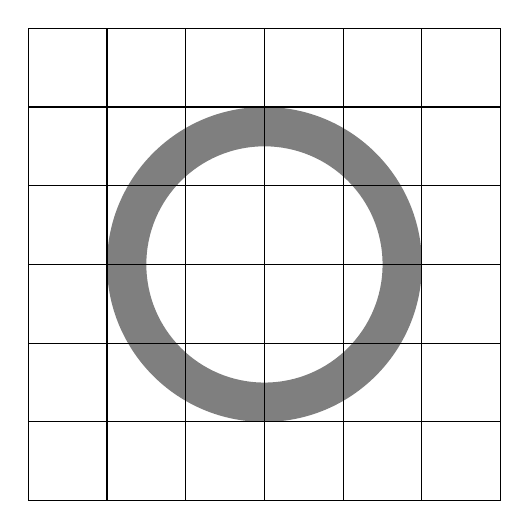
\begin{tikzpicture}                    \draw (0,0) grid (6,6);
                    %\fill [orange] (1,1) rectangle (2,2);
                        \fill [even odd rule, opacity=0.5] 
                        (3,3) circle [radius=2] circle [radius=1.5];
                    \end{tikzpicture}
            }
         \caption{Top-down view}
    \end{subfigure}
    \caption{BEV image generated by IPM}
    \label{fig:ipm}
\end{figure}

%The application of the IPM transform
%requires the knowledge of the camera specific acquisition conditions and some assumption on the scene %represented in the image (here defined as a priori knowledge).\\

In general, the perspective transformation can be expressed as 
\begin{equation}
p' =  \textbf{G} p
\label{eq:ipm}
\end{equation} 
where \textbf{G} can be expressed in terms of the
intrinsic matrix \textbf{K} and the Euclidean \textbf{homography} matrix
$\textbf{H} \in \mathbb{SL}(3)$ related to a planar viewed object. It should be noted that $\textbf{H}$
depends on the rotation matrix $\textbf{R}$ and the translation vector
$\textbf{t}$ corresponding to the rigid transformation between the real camera pose image and generated one.\\

IPM can be conveniently computed automatically~\cite{hom_single, adaptive_ipm} or constructed using scene measurements, satellite images from  publicly available map services (e.g. Google Maps).

\subsection{Object detection and tracking}

 
 \newsavebox{\cube}
    \begin{lrbox}{\cube}
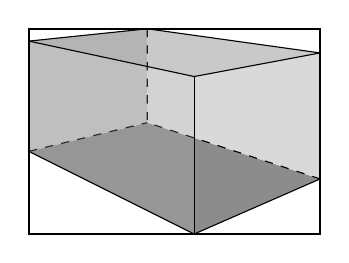
\begin{tikzpicture}
%\draw (-3,-2) grid (2,1);
%\fill [green, even odd rule, opacity=0.5] 
%(-0.5,-0.5) circle [radius=1.3] circle [radius=1];

	%%% Edit the following coordinate to change the shape of your
	%%% cuboid
      
	%% Vanishing points for perspective handling
	\coordinate (P1) at (-7cm,1.5cm); % left vanishing point (To pick)
	\coordinate (P2) at (8cm,1.5cm); % right vanishing point (To pick)

	%% (A1) and (A2) defines the 2 central points of the cuboid
	\coordinate (A1) at (0em,0cm); % central top point (To pick)
	\coordinate (A2) at (0em,-2cm); % central bottom point (To pick)

	%% (A3) to (A8) are computed given a unique parameter (or 2) .8
	% You can vary .8 from 0 to 1 to change perspective on left side
	\coordinate (A3) at ($(P1)!.7!(A2)$); % To pick for perspective 
	\coordinate (A4) at ($(P1)!.7!(A1)$);

	% You can vary .8 from 0 to 1 to change perspective on right side
	\coordinate (A7) at ($(P2)!.8!(A2)$);
	\coordinate (A8) at ($(P2)!.8!(A1)$);

	%% Automatically compute the last 2 points with intersections
	\coordinate (A5) at
	  (intersection cs: first line={(A8) -- (P1)},
			    second line={(A4) -- (P2)});
	\coordinate (A6) at
	  (intersection cs: first line={(A7) -- (P1)}, 
			    second line={(A3) -- (P2)});

    %\path let \p1=(A2) in
     %   coordinate (W1) at (0,\y1); % point on y-axis

    \path let \p1=(A5) in
        coordinate (W2) at (0,\y1); % point on y-axis


	\coordinate (C1) at
	  (intersection cs: first line={(A4) -- (A3)}, 
			    second line={(A2) -- (1em,-2cm)});
	\coordinate (C2) at
	  (intersection cs: first line={(A8) -- (A7)}, 
			    second line={(A2) -- (1em,-2cm)});
			    
	\coordinate (C3) at
	  (intersection cs: first line={(W2) -- (A5)}, 
			    second line={(A7) -- (A8)});
			    

	%%% Depending of what you want to display, you can comment/edit
	%%% the following lines

	%% Possibly draw back faces

	\fill[gray!90] (A2) -- (A3) -- (A6) -- (A7) -- cycle; % face 6
	%\node at (barycentric cs:A2=1,A3=1,A6=1,A7=1) {\tiny f6};
	
	\fill[gray!50] (A3) -- (A4) -- (A5) -- (A6) -- cycle; % face 3
	%\node at (barycentric cs:A3=1,A4=1,A5=1,A6=1) {\tiny f3};
	
	\fill[gray!30] (A5) -- (A6) -- (A7) -- (A8) -- cycle; % face 4
	%\node at (barycentric cs:A5=1,A6=1,A7=1,A8=1) {\tiny f4};
	
	\draw[dashed] (A5) -- (A6);
	\draw[dashed] (A3) -- (A6);
	\draw[dashed] (A7) -- (A6);

	%% Possibly draw front faces

	% \fill[orange] (A1) -- (A8) -- (A7) -- (A2) -- cycle; % face 1
	% \node at (barycentric cs:A1=1,A8=1,A7=1,A2=1) {\tiny f1};
	\fill[gray!50,opacity=0.2] (A1) -- (A2) -- (A3) -- (A4) -- cycle; % f2
	%\node at (barycentric cs:A1=1,A2=1,A3=1,A4=1) {\tiny f2};
	\fill[gray!90,opacity=0.2] (A1) -- (A4) -- (A5) -- (A8) -- cycle; % f5
	%\node at (barycentric cs:A1=1,A4=1,A5=1,A8=1) {\tiny f5};

	%% Possibly draw front lines
	\draw (A1) -- (A2);
	\draw (A3) -- (A4);
	\draw (A7) -- (A8);
	\draw (A1) -- (A4);
	\draw (A1) -- (A8);
	\draw (A2) -- (A3);
	\draw (A2) -- (A7);
	\draw (A4) -- (A5);
	\draw (A8) -- (A5);
	
	% Possibly draw points
	% (it can help you understand the cuboid structure)
	%\foreach \i in {1,2,...,8}
	%{
	 % \draw[fill=black] (A\i) circle (0.15em)
	%    node[above right] {\tiny A\i};
	%}
	%\draw[fill=green] (P1) circle (0.1em) node[below] {\tiny p1};
	%\draw[fill=green] (P2) circle (0.1em) node[below] {\tiny p2};

	%\draw[fill=red] (C1) circle (0.2em) node[below] {\tiny C1};
	%\draw[fill=red] (C2) circle (0.2em) node[below] {\tiny C2};
	%\draw[fill=red] (C3) circle (0.2em) node[below] {\tiny C3};
	
	%\draw[fill=green] (W1) circle (0.2em) node[below] {\tiny W1};
	
	%draw[thick, red] (A4) -- (C1);
	%\draw[thick, red] (C1) -- (C2);
	%\draw[thick] (C2) -- (A8);
    \draw[thick] (C1) rectangle (C3);
    %\draw[thick, green] (C1) rectangle ++(0.3,0.3);
\end{tikzpicture}
\end{lrbox}

\newsavebox{\icube}
    \begin{lrbox}{\icube}
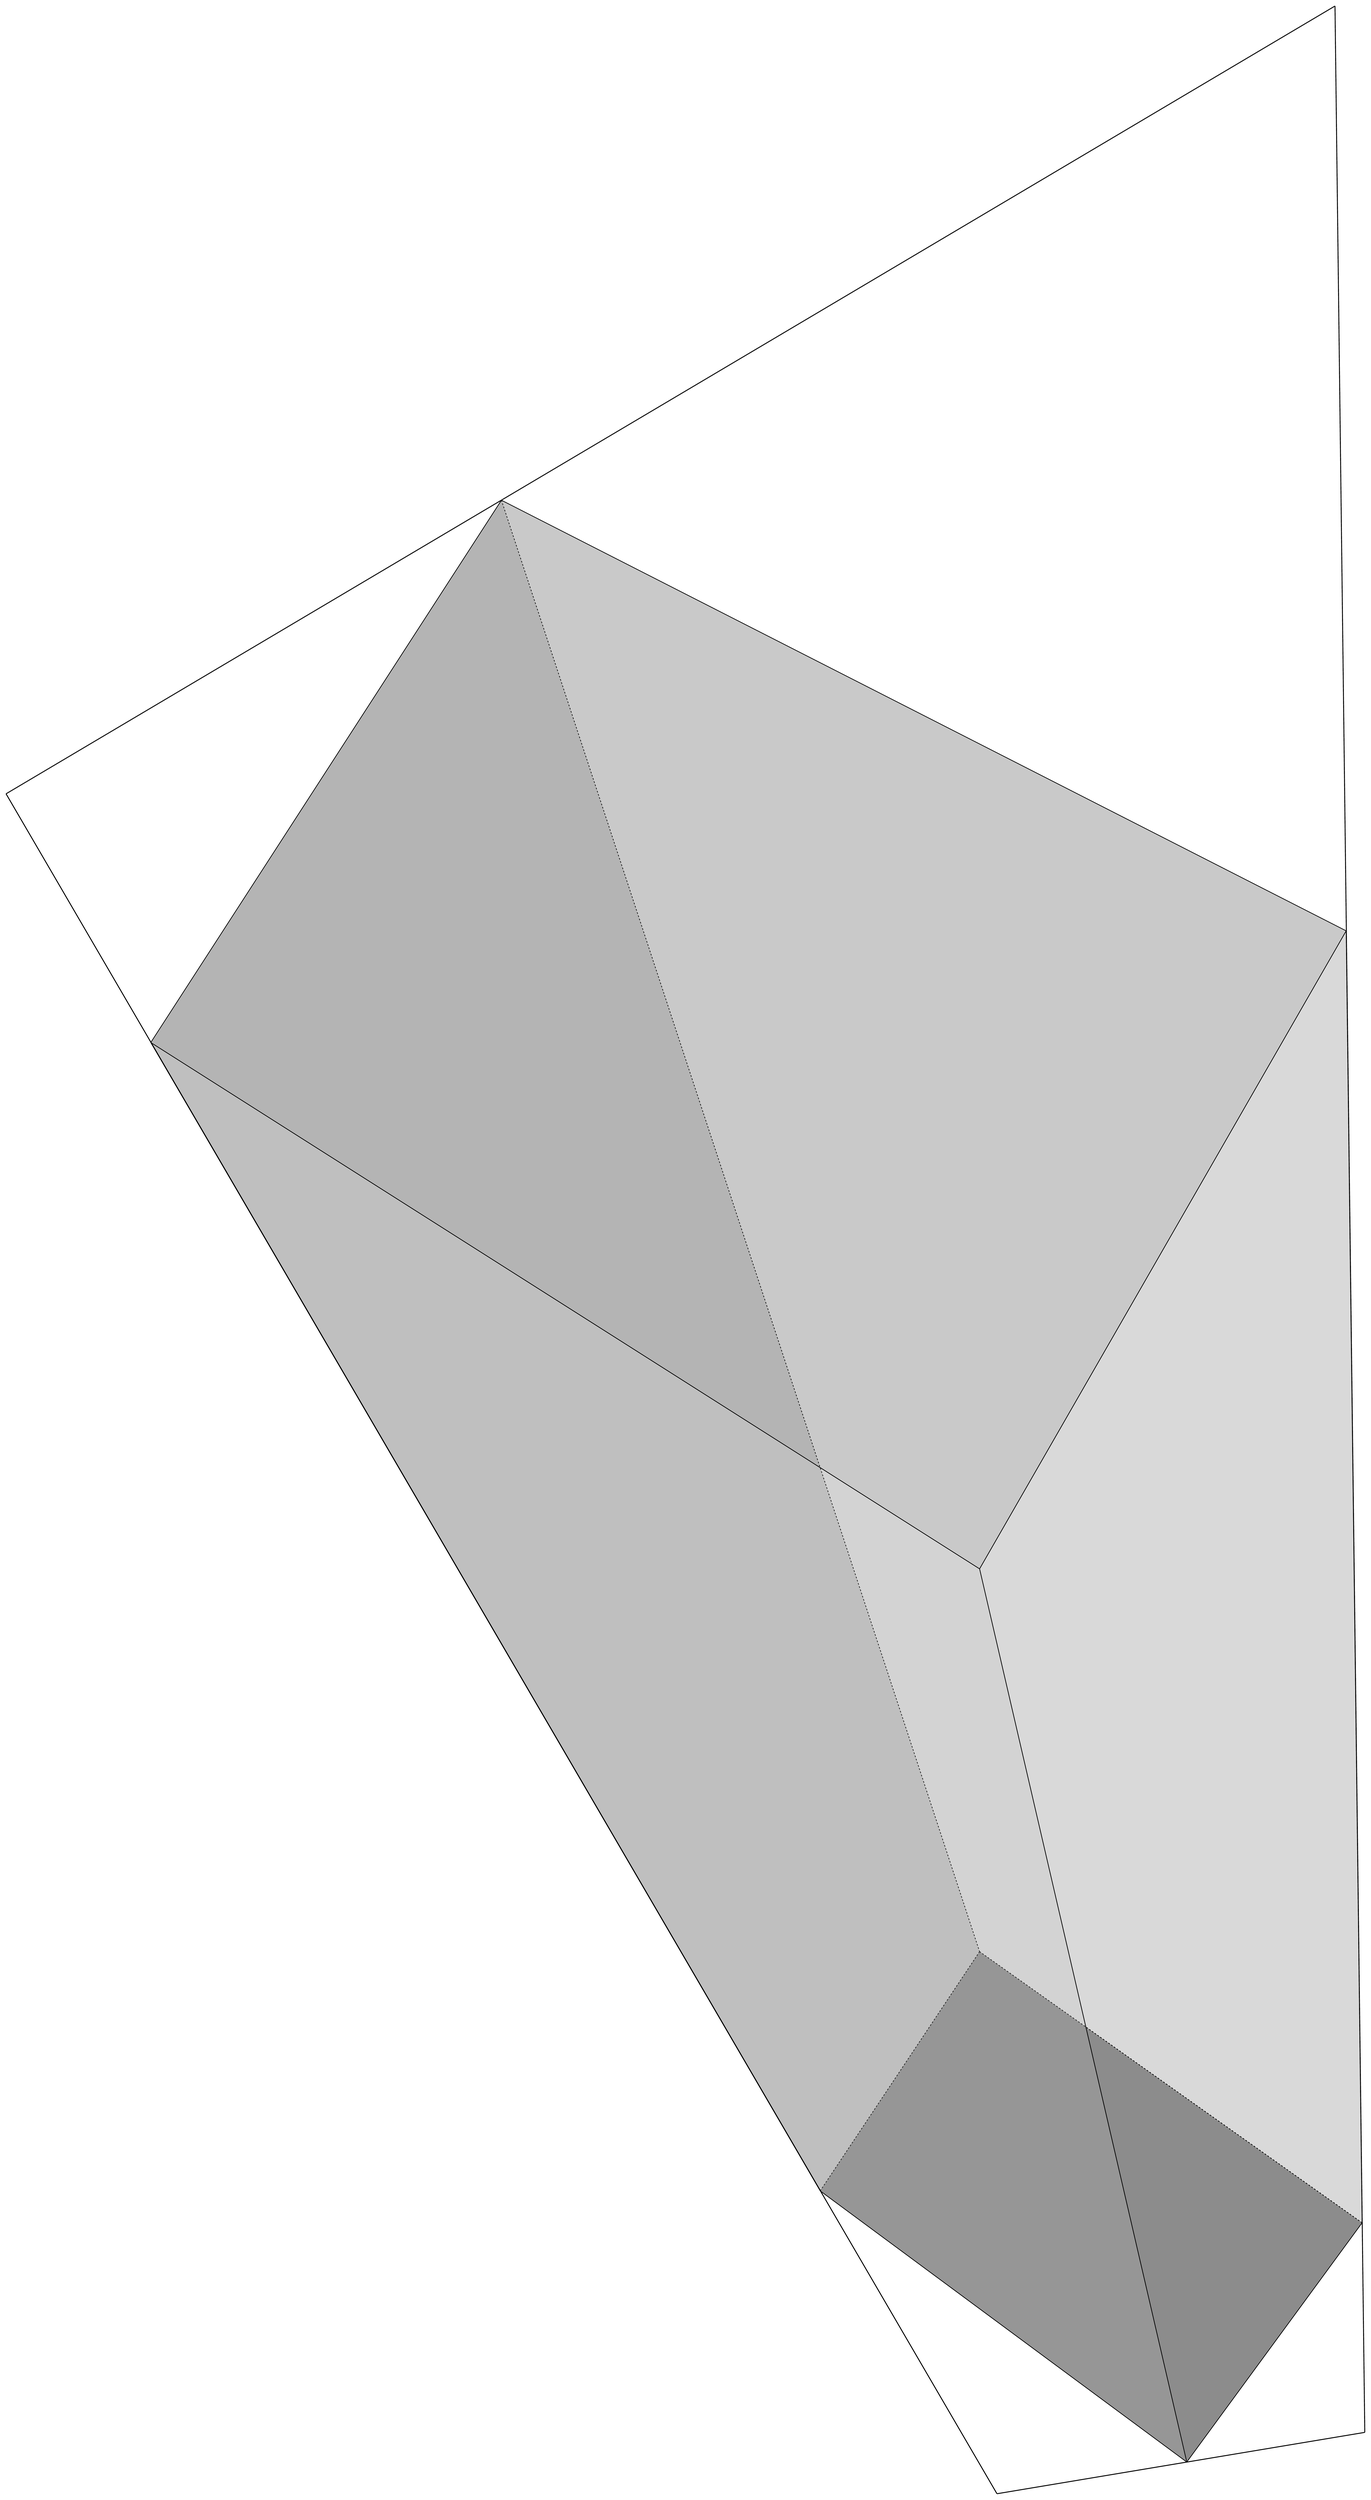
\begin{tikzpicture}

	%% (A1) and (A2) defines the 2 central points of the cuboid
	% 3173
	%\coordinate (A1) at (126cm,57cm); % central top point (To pick)
	\coordinate (A1) at (127cm, 60); %68); %58cm);
	\coordinate (A2) at (140cm,4cm); % central bottom point (To pick)
	\coordinate (A3) at (117cm,21cm);
	\coordinate (A4) at (75cm,93cm); %(79cm,93cm);
	\coordinate (A5) at (97cm,127cm);
	\coordinate (A6) at (127cm,36cm);
	%\coordinate (A7) at (151cm,20cm);
	\coordinate (A7) at (151cm,19cm);
	\coordinate (A8) at (150cm, 100); %(148cm, 104); %106cm);
	
	%\coordinate (C1) at (127cm,2cm);
	\coordinate (C2) at (70cm,111cm);
	
	\coordinate (C3) at (148cm,156cm);
	\coordinate (C4) at (152cm,6cm);
	\coordinate (C1) at
	  (intersection cs: first line={(A2) -- (C4)}, 
			    second line={(A3) -- (A4)});
	\coordinate (C4) at
	  (intersection cs: first line={(A2) -- (C4)}, 
			    second line={(A8) -- (A7)});
	\coordinate (C2) at
	  (intersection cs: first line={(A5) -- (C2)}, 
			    second line={(A3) -- (A4)});
	\coordinate (C3) at
	  (intersection cs: first line={(A5) -- (C2)}, 
			    second line={(A7) -- (A8)});

	%% Possibly draw back faces

	\fill[gray!90] (A2) -- (A3) -- (A6) -- (A7) -- cycle; % face 6
	%\node at (barycentric cs:A2=1,A3=1,A6=1,A7=1) {\tiny f6};
	
	\fill[gray!50] (A3) -- (A4) -- (A5) -- (A6) -- cycle; % face 3
	%\node at (barycentric cs:A3=1,A4=1,A5=1,A6=1) {\tiny f3};
	
	\fill[gray!30] (A5) -- (A6) -- (A7) -- (A8) -- cycle; % face 4
	%\node at (barycentric cs:A5=1,A6=1,A7=1,A8=1) {\tiny f4};
	
	\draw[very thick,dashed] (A5) -- (A6);
	\draw[very thick,dashed] (A3) -- (A6);
	\draw[very thick,dashed] (A7) -- (A6);

	%% Possibly draw front faces

	% \fill[orange] (A1) -- (A8) -- (A7) -- (A2) -- cycle; % face 1
	% \node at (barycentric cs:A1=1,A8=1,A7=1,A2=1) {\tiny f1};
	\fill[gray!50,opacity=0.2] (A1) -- (A2) -- (A3) -- (A4) -- cycle; % f2
	%\node at (barycentric cs:A1=1,A2=1,A3=1,A4=1) {\tiny f2};
	\fill[gray!90,opacity=0.2] (A1) -- (A4) -- (A5) -- (A8) -- cycle; % f5
	%\node at (barycentric cs:A1=1,A4=1,A5=1,A8=1) {\tiny f5};

	%% Possibly draw front lines
	\draw[very thick] (A1) -- (A2);
	\draw[very thick] (A3) -- (A4);
	\draw[very thick] (A7) -- (A8);
	\draw[very thick] (A1) -- (A4);
	\draw[very thick] (A1) -- (A8);
	\draw[very thick] (A2) -- (A3);
	\draw[very thick] (A2) -- (A7);
	\draw[very thick] (A4) -- (A5);
	\draw[very thick] (A8) -- (A5);
	
	\draw[ultra thick] (C1) -- (C2);
	\draw[ultra thick] (C2) -- (C3);
	\draw[ultra thick] (C3) -- (C4);
	\draw[ultra thick] (C4) -- (C1);
	
	%\MarkRightAngle{A7}{A2}{A3}
\end{tikzpicture}
\end{lrbox}
 

2D Object Detection is a common Computer Vision technique for identifying and locating objects of certain classes in the image.
A 2D bounding box (rectangle) is used to describe the location of an object. It is determined by the  rectangle center $C = (c_x, c_y)$, dimension $D = (d_x, d_y) $ with the width and height of the rectangle and type of the object $T$. The example of 2d detection using YOLO (You Only Look Once) algorithm is shown in Fig.~\ref{fig:klichko}.


\begin{figure}%[h]
    \centering
    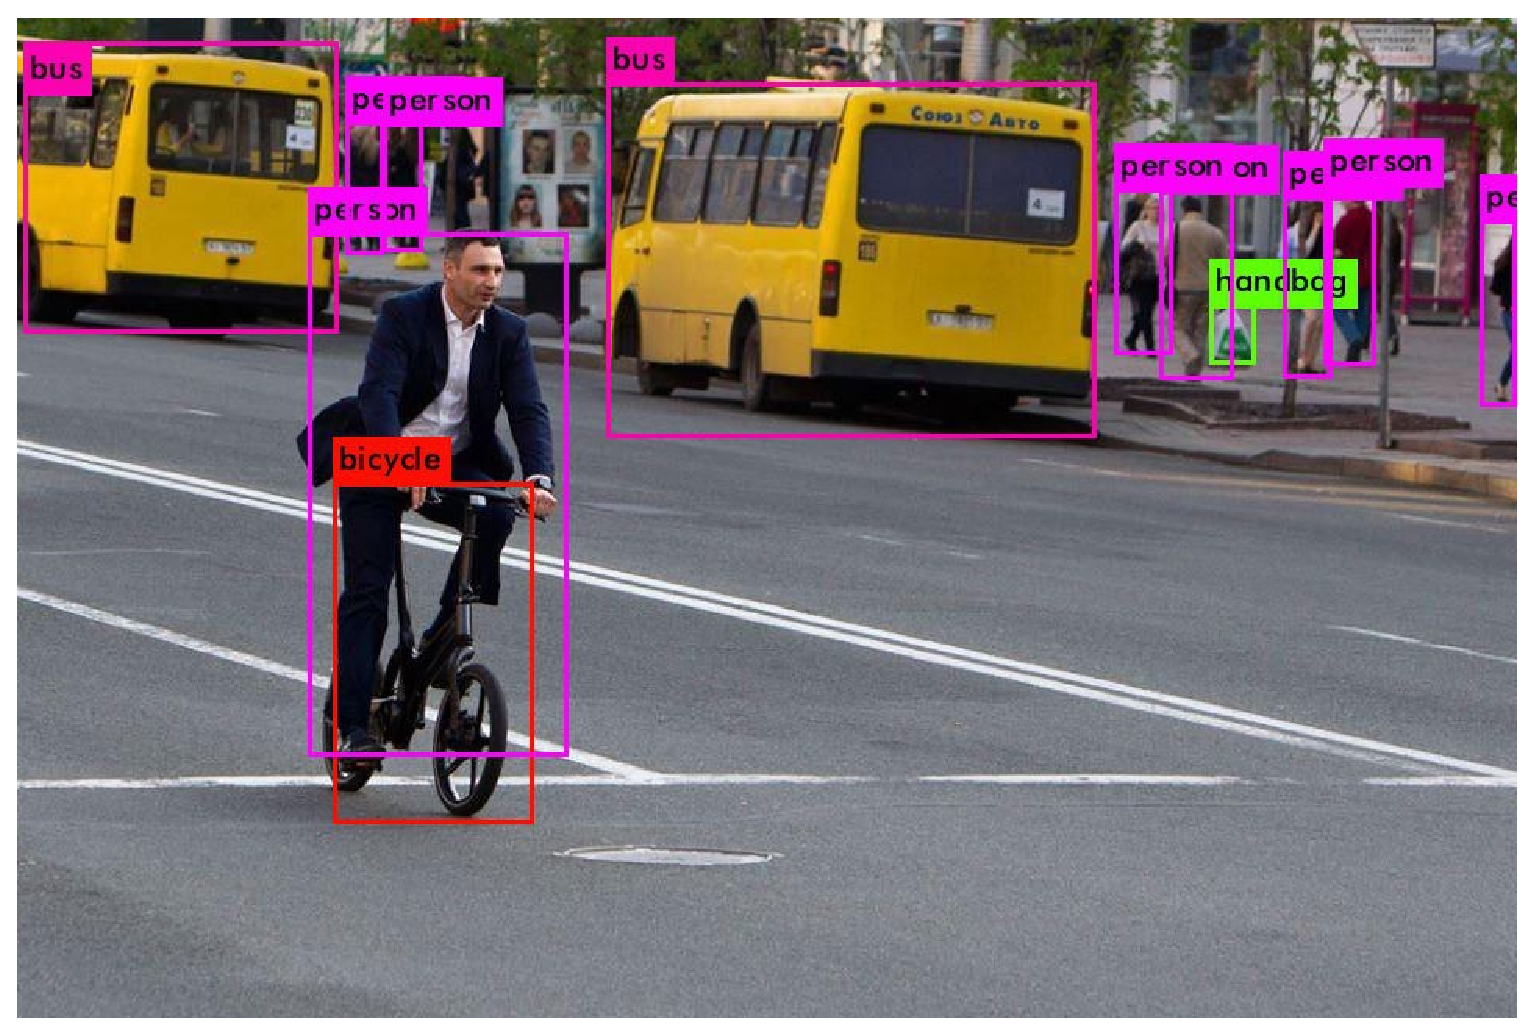
\includegraphics[width=0.8\textwidth]{KlichkoColor.eps}
    \caption{2D object detection and classification with YOLOv3}
    \label{fig:klichko}
\end{figure}

\textbf{Multi-Object Tracking} (MOT)~\cite{kalman_mot} is mainly used in videos to determine whether objects recognized in consecutive frames are the same or not and to track the path of movement in the case of the same objects.
It produces a set of trajectories based on a video frame $f$ and an object $o$ center detection as they move around.

In the case of \textbf{3D detection}, the bounding cuboid (or rectangular parallelepiped) is described by its 
center $C = (c_x, c_y, c_z)$, dimensions $D = (d_x, d_y, d_z)$, and
orientation $R = (\varphi, \theta, \psi)$ parameterized  by elevation, azimuth, and roll angles.


\section{Proposed method}  \label{sec:meth}
Existing 2D detectors not only build a bounding box around the object but also allow it to be classified. For example, vehicles can be classified by body type. That makes it possible to get their average size as shown in Table~\ref{table_sizes}. Moreover, using the classification by model~\cite{model_det}, we get the exact dimensions of the object from \url{https://www.automobiledimension.com}. %For our method, it does not matter how the dimensions are obtained. Both options can be used. 
In the case of classification by model, the orientation will be determined exactly, and in other  cases, with some error, which will be described below.

We will also use the directions of motion of the 2D detection box centers, that do not coincide with the movement of the object itself. However, a method for correction will be suggested.


The basic idea of the proposed method is to find object bottom box projection on the BEV using object sizes and moving direction. Further, it will be shown how, using the detected boxes and object sizes, to calculate the possible orientations and choose the one that best suits the movement of the object.

\begin{table}%[h!]
\caption{Vehicle categories and their average dimensions}
\centering
\begin{tabular}{ |p{3cm}||p{4cm}|p{2cm}|p{2cm}|  }
 \hline
 %\multicolumn{4}{|c|}{Country List} \\
 %\hline
Category & Vehicles included & Length (m) & Width (m) \\
 \hline
 Car & Car, jeep & 3.72 & 1.44\\
 Bus & Bus & 10.1 & 2.43\\
 Truck & Truck & 7.5 & 2.35\\
 LCV & Mini bus, vans & 6.1 & 2.10 \\
Tractor & Tractor, trailer & 7.4 & 2.20\\
 Three-wheeler & Three wheeler & 3.2 & 1.40\\
 Two-wheeler & Scooter, motorbike & 1.87 & 0.64\\
 Cycle & Bicycles & 1.9 & 0.45\\
 \hline
\end{tabular}
\label{table_sizes}
\end{table}

%Table~\ref{table_sizes} provides average sizes for each type of vehicle category used in this article.

%We do not only get advantage of the robust performance of existing 2D detectors to generate classified 2D bounding boxes but also, using the classification by model~\cite{model_det}, we get the dimensions of the object from \url{https://www.automobiledimension.com}. At least we will know the average dimensions of a vehicle using the classification by body type. In this case, we can get some error in determining the orientation and we will show its estimate.



\begin{figure}%[h]
    \centering
    \begin{subfigure}[t]{0.4\textwidth}
        \centering
                 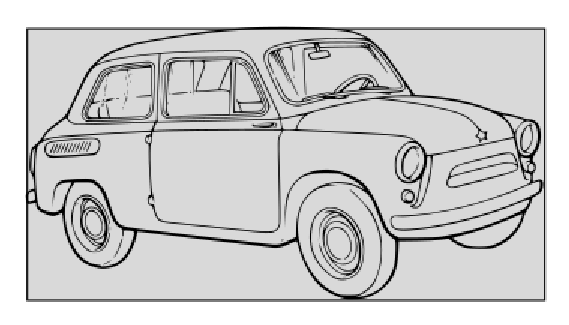
\includegraphics[width = \textwidth]{zaz_2d.eps}
        \caption{2D detection}
    \end{subfigure}%
    ~ 
    \begin{subfigure}[t]{0.4\textwidth}
        \centering
           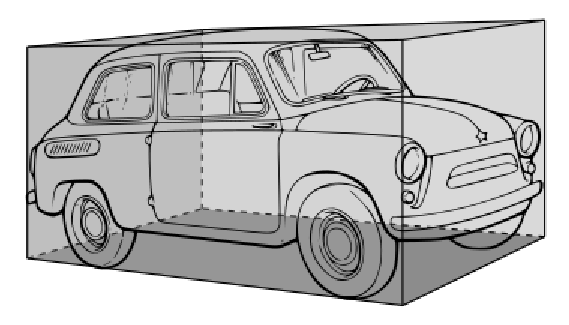
\includegraphics[width = \textwidth]{zaz_3d.eps}
         \caption{3D detection}
    \end{subfigure}
    \caption{Vehicle detection}
    \label{fig:detection}
\end{figure}


\subsection{Model assumptions}
Our main task is to detect vehicles on the road and parking lot, but it is not limited to this application.
Several assumptions have been made in order to build a mathematical model. 
We are most interested in the planar position of the objects and  assume a
vehicle is always on the (flat) ground. %and camera distortion is negligible.
It allows assuming that only the azimuth (noted $\theta$) matters and thus we do not predict the orientation $R$ characterized by  elevation and roll and we set $\varphi = 0$ and $\psi = 0$.\\

The camera position must be stationary. In another case, object moving vectors obtained from MOT have to be recalculated.
And the vehicle being detected must be attached to the plane of the ground because only the points on the ground have the distance information.  



%This coincides with the definition of 3D detection and does not contradict to the \textbf{Manhattan World assumption}[ref] which states that most human-made structures could be approximated by planar surfaces that are parallel to one of the three principal planes of a common orthogonal coordinate system.

%As commonly done in vehicle-oriented applications, we assume object pitch φ
%and roll α angles are zeros
In the context of our model, we will use a cuboid approximation of a 3D object which coincides with the definition of 3D detection as shown in Fig.~\ref{fig:detection}.
We assume that 3D detection perfectly fits into 2D detection. Therefore at least one vertex of the bottom box  lies on the lower side of the 2D detection rectangle. Accordingly, we can see a similar situation in BEV as shown in Fig.~\ref{fig:ipm_cube}.\\





%In this work we assume that scene is flat and its dimensions are known. It allows to produce BEV image using Equation~\ref{eq:ipm} with known sizes of the flat objects on it.\\

Further, we will show how to find the projection of the lower face of the cuboid in  BEV.
This makes it possible to determine the orientation and center of the cuboid with known sizes. It should be noted that the orientation of the object is set up to the opposite since we do not geometrically distinguish between the front and back of a vehicle, which is appropriate in the case of cars since they can go both forward and backward, but not sidewards.

\subsection{Bottom box determination} \label{sec:comp}
All calculations that are given in this section will refer to calculations in BEV. The domain of an IPM is an image with 2D objects detection.\\

\begin{figure}%[h]
    \centering
    \begin{subfigure}[t]{0.4\textwidth}
        \centering
            \resizebox{.9\textwidth}{!}{%
                 \usebox{\cube}
            }
        \caption{Cube 2D detection}
    \end{subfigure}%
    ~ 
    \begin{subfigure}[t]{0.4\textwidth}
 
         \resizebox{.6\textwidth}{!}{%
            \usebox{\icube}
            }
         \caption{IPM transformation}
    \end{subfigure}
    \caption{IPM of the 2D detection}
    \label{fig:ipm_cube}
\end{figure}


Let the IPM image of an object detection rectangle  will be non-degenerate quadrangle $A, R, T, B$ with an inner rectangle whose three vertices lie on adjacent sides. Moreover, one of the vertices of the rectangle lies on the bottom side of the outer quadrangle as shown in Fig.~\ref{fig:bottom}. Our goal is to find touchpoints $K, C, D$, and angle $\varphi$. Further we will refer to such quadrangles as \textbf{bounding} ones. Under these conditions, we will prove the following statements.


\begin{figure}%[H]
    \centering

\resizebox{0.5\textwidth}{!}{%
\begin{tikzpicture}

    %\draw (0,0) grid (10,15);

    \coordinate (A1) at (2cm,0cm);
    \coordinate (A4) at (8cm,1cm);
    \coordinate (A2) at (0cm,10cm); %(0cm,13cm);
    \coordinate (A3) at (10cm,11cm); %(10cm,15cm);
    
    \coordinate (K) at (0,9cm);
    \coordinate (C) at (6,0cm);
    \coordinate (C1) at (0,6cm);
    \coordinate (D) at (10,2cm);
    \coordinate (D1) at (0,13cm);
    
    \coordinate (K) at
	  (intersection cs: first line={(A4) -- (K)}, 
			    second line={(A1) -- (A2)});
			    
	\coordinate (C) at
	  (intersection cs: first line={(A1) -- (A4)}, 
			    second line={(C) -- (C1)});
	\coordinate (B) at
	  (intersection cs: first line={(C) -- (C1)}, 
			    second line={(A1) -- (A2)});
	
	\coordinate (D) at
	  (intersection cs: first line={(A4) -- (A3)}, 
			    second line={(D1) -- (D)});
			    
			    

	\draw[fill=black] (A1) circle (0.15em)
	    node[below left] {A};
	\draw[fill=black] (A4) circle (0.15em)
	    node[above right] {B};
	\draw[fill=black] (A2) circle (0.15em)
	    node[above left] {R};
	\draw[fill=black] (A3) circle (0.15em)
	    node[above right] {T};
	

    \draw[fill=black] (K) circle (0.15em) node[above left] {E};
    
    \draw[fill=black] (C) circle (0.15em) node[below left] {C};
    
    \draw[fill=black] (D) circle (0.15em) node[above right] {D};
    \draw[fill=black] (B) circle (0.15em) node[above left] {K};


%	\draw[thick] (A1) -- (A4);
%	\draw[thick] (A4) -- (A3);
%	\draw[thick] (A3) -- (A2);
%	\draw[thick] (A1) -- (A2);


	\draw[thick] (A1) -- (A4);
	\draw[thick] (A4) -- (A3);
	\draw[thick] (A3) -- (A2);
	\draw[thick] (A1) -- (A2);
	
	\draw[thick] (C) -- (D);
	\draw[thick] (C) -- (B);
	
	\draw[thick, dashed] (A4) -- (K);

    \MarkRightAngle{D}{C}{B}
    \draw pic["$\varphi$", draw=black, -, angle eccentricity=1.2, angle radius=1cm]
    {angle=K--A4--C};
    

    \draw pic["$\varphi$", draw=black, -, angle eccentricity=1.2, angle radius=1cm]
    {angle=B--C--A1};


\end{tikzpicture}
}

    \caption{Rectangle reconstruction by angle and sizes}
    \label{fig:bottom}
\end{figure}

\begin{proposition} \label{prop:orient}
%A cuboid with known dimensions and orientation can be reconstructed from BEV image with rectangular detection.
%\\
A rectangle with known dimensions and orientation can be reconstructed from bounding quadrangle.
\end{proposition}
\begin{proof}
Let the rectangle be built on points $K$, $C$, and $D$ with fixed sizes $KC = a$ and $CD = b$ as shown in Fig.~\ref{fig:bottom}.
Let us draw a ray from $B$ with the angle equal to the orientation. We denote $E$ the intersection point of this ray with segment $AR$,  and $\angle ABE = \varphi$, and let $EB = l$. According to the construction  $\triangle K A C \backsim  \triangle E A B$ and 
from the similarity we have 
$\dfrac{AC}{AB} = \dfrac{KC}{EB} = \dfrac{a}{l}$.\\
Hereof $AC = \dfrac{a}{l} (AC + CB)$ and $AC  = \dfrac{a}{l-a} CB$.\\
Consequently $C= (C_x, C_y) = \left(\dfrac{(l - a) A_x + a  B_x}{l}, \dfrac{(l - a) A_y + a B_y}{l}\right)$ which makes it possible to recover the rectangle. 

\begin{comment}
%Let a rectangle that is fixed at points with sides 1 and 2.
%with known sizes $(l_replace, a)$ and $\angle KCD = \frac{\pi}{2}$.



$$\overline{A_1 C} = \frac{a}{l} (\overline{A_1 C} + \overline{C A_4}) $$
$$\left(1 - \frac{a}{l}\right) \overline{A_1 C} = \frac{a}{l} \overline{C A_4} $$
$$ \overline{A_1 C}  = \frac{a}{l-a} \overline{C A_4} $$

$$C = (C_x, C_y) = \left(\frac{(l - a) x_1 + a  x_4}{l}, \frac{(l - a) y_1 + a y_4}{l}\right)$$

This equation shows that the bottom projection rectangle can be determined from the BEV image.

\end{comment}
\end{proof}


\begin{figure}%[h]
    \centering

\resizebox{0.5\textwidth}{!}{%
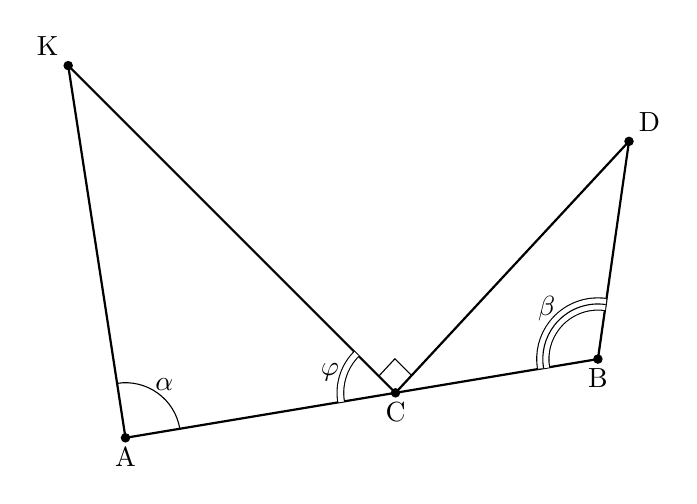
\begin{tikzpicture}[double arc/.style={double,double distance=2pt},
 triple arc/.style={double distance=4pt,
    pic actions/.append code=\tikzset{postaction={draw}}}]

    %\draw (0,0) grid (10,15);

    \coordinate (A1) at (2cm,0cm);
    \coordinate (A4) at (8cm,1cm);
    \coordinate (A2) at (0cm,13cm);
    \coordinate (A3) at (10cm,15cm);
    
    \coordinate (K) at (0,9cm);
    \coordinate (C) at (6,0cm);
    \coordinate (C1) at (0,6cm);
    \coordinate (D) at (10,2cm);
    \coordinate (D1) at (0,13cm);
    
    \coordinate (K) at
	  (intersection cs: first line={(A4) -- (K)}, 
			    second line={(A1) -- (A2)});
			    
	\coordinate (C) at
	  (intersection cs: first line={(A1) -- (A4)}, 
			    second line={(C) -- (C1)});
	\coordinate (B) at
	  (intersection cs: first line={(C) -- (C1)}, 
			    second line={(A1) -- (A2)});
	
	\coordinate (D) at
	  (intersection cs: first line={(A4) -- (A3)}, 
			    second line={(D1) -- (D)});
			    
			    

     \draw[fill=black] (A1) circle (0.15em)
	    node[below] {A};
     \draw[fill=black] (A4) circle (0.15em)
	    node[below] {B};
	

    \draw[fill=black] (C) circle (0.15em) node[below] {C};
    
    \draw[fill=black] (D) circle (0.15em) node[above right] {D};
    \draw[fill=black] (B) circle (0.15em) node[above left] {K};

	\draw[thick] (A1) -- (A4);
	\draw[thick] (D) -- (A4);
	%\draw[thick] (A3) -- (A2);
	\draw[thick] (A1) -- (B);
	
	\draw[thick] (C) -- (D);
	\draw[thick] (C) -- (B);
	

    \MarkRightAngle{D}{C}{B}
    \draw pic[draw, "$\beta$", triple arc, angle eccentricity=1.3, angle radius=0.7cm]  {angle=A3--A4--A1};


    \draw pic[draw, "$\varphi$", double arc, -, angle eccentricity=1.25, angle radius=0.7cm]
    {angle=B--C--A1};
    \draw pic["$\alpha$", draw=black, -, angle eccentricity=1.2, angle radius=0.7cm]
    {angle=C--A1--B};


\end{tikzpicture}
}

    \caption{Fixed sizes rectangle fitting}
    \label{fig:bottom_variants}
\end{figure}

\begin{theorem}
\label{th:restriction}
There are at most 4 possibilities to fit  a rectangle into a bounding quadrangle.
\end{theorem}
\begin{proof}
Suppose we have bounding quadrangle with fixed $KC = a$, $CD = b$, $AB = d$, $\angle KAC = \alpha$, and $\angle CBD = \beta $ as shown in Fig.~\ref{fig:bottom_variants}. To distinguish between different fitting possibilities let us assume that $a \geq b$.
According to the sine rule
\begin{gather*} 
\frac{a}{\sin{\alpha}} = \frac{AC}{\sin{(\alpha + \varphi)}}\\ 
\frac{b}{\sin{\beta}} = \frac{BC}{\sin{(\beta + \frac{\pi}{2}- \varphi)}}
\end{gather*}
\begin{comment}
$$AC = \frac{a\sin{(\alpha + \varphi)}}{\sin{\alpha}}, BC = \frac{b \sin{(\frac{\pi}{2} + \beta - \varphi)}}{\sin{\beta}} = \frac{b \cos{(\beta - \varphi)}}{\sin{\beta}}$$
\end{comment}

As a result $ AC + BC =  \dfrac{a\sin{(\alpha + \varphi)}}{\sin{\alpha}} + \dfrac{b \cos{(\beta - \varphi)}}{\sin{\beta}} = d$ \\
and consequently we obtain the following equation:
\begin{multline}\label{sin_eq}
(a \sin \beta \sin \alpha + b \sin \alpha \cos \beta) \cos \varphi + \\
(a \sin \beta \cos \alpha + b \sin \alpha \sin \beta) \sin \varphi = d \sin \alpha \sin \beta
\end{multline}

%$$ a \sin{\beta}(\sin \alpha \cos \alpha) + b \sin \alpha (\cos \beta \cos \varphi + \sin \beta \sin \alpha)  = d \sin \alpha \sin \beta$$
%$$(a \sin \beta \sin \alpha + b \sin \alpha \cos \beta) \cos \varphi + (a \sin \beta \cos \alpha + b \sin \alpha \sin \beta) \sin \varphi = d \sin \alpha \sin \beta$$

Let us denote
\begin{gather*}
e = a \sin \beta \sin \alpha + b \sin \alpha \cos \beta = \sin \alpha ( a \sin \beta + b \cos \beta)\\ 
 f = a \sin \beta \cos \alpha + b \sin \alpha \sin \beta = \sin \beta ( a \cos \alpha + b \sin \alpha)\\
 g = d \sin \alpha \sin \beta > 0
\end{gather*}
In terms of these notations, we get the equality $e \cos \varphi + f \sin \varphi = g$.\\
Further, if we denote $\dfrac{e}{\sqrt{e^2 + f^2}} = \cos \theta$ and $\dfrac{f}{\sqrt{e^2 + f^2}} = \sin \theta$, where $0 \leq \theta < 2 \pi$
, then we get that $\cos{(\varphi - \theta)} = \dfrac{g}{\sqrt{e^2 + f^2}}$.\\
Hence we obtain that 
\begin{equation} \label{eq:phi}
\varphi = \theta \pm \psi + 2 \pi n
\end{equation}
where $\psi = \arccos{\dfrac{g}{\sqrt{e^2 + f^2}}}$ and $0 \leq \psi < \frac{\pi}{2}$.
\end{proof}

\begin{comment}

$ e^2 + f^2 =  \sin^2 \alpha ( a \sin \beta + b \cos \beta)^2 + \sin ^2 \beta ( a \cos \alpha + b \sin \alpha)^2 = a^2 \sin ^ 2 \beta + b^2 \sin ^2 \alpha + 2ab \sin \alpha \sin \beta \sin{(\alpha + \beta)} \\
e \cos \varphi + f \sin \varphi = e
$
$$ \frac{e}{\sqrt{e^2 + f^2}} \cos \varphi + \frac{f}{\sqrt{e^2 + f^2}} \sin \varphi = \frac{g}{\sqrt{e^2 + f^2}}$$
$\frac{e}{\sqrt{e^2 + f^2}} = \cos \theta, \frac{f}{\sqrt{e^2 + f^2}} = \sin \theta$, where $0 \leq \theta < 2 \pi$
$\cos \theta cos\varphi + \sin \theta \cos \varphi = \frac{g}{\sqrt{e^2 + f^2}}$,
$\cos{(\varphi - \theta)} = \frac{g}{\sqrt{e^2 + f^2}}$ $0 < g \leq \sqrt{e^2 + f^2}$

$\varphi - \theta = \pm \arccos{\frac{g}{\sqrt{e^2 + f^2}}} + 2 \pi n$ \\
Let $\psi = \arccos{\frac{g}{\sqrt{e^2 + f^2}}}$, $0 \leq \psi < \frac{\pi}{2}$\\


\begin{equation} \label{eq:phi}
\varphi = \theta \pm \psi + 2 \pi n
\end{equation}
\end{comment}


\begin{remark}
At least one solution exists by definition.
\end{remark}

\begin{remark}
The proposition presented below not only restricts the number of possible object orientations but also shows the way of the bottom rectangle reconstruction.
\end{remark}


\begin{figure}%[h]
    \centering

\resizebox{0.5\textwidth}{!}{%
% 5 3

\begin{tikzpicture}[double arc/.style={double,double distance=2pt},
 triple arc/.style={double distance=4pt,
    pic actions/.append code=\tikzset{postaction={draw}}}]

 \draw [<->] (0,6) node (yaxis) [above] {$y$}
        |- (4,0) node (xaxis) [right] {$x$};   

% \draw (-6,-6) grid (6,6);
         \tikzmath{
            \a = 5;
            \b = 3;
            \angl = 75;
            coordinate \q1, \q2;
            \q1 = ({ - (\a)/2 * 1/tan(\angl)}, \a/2);
            \q2 = (\b/2,  {- (\b)/2 * 1/tan(\angl)});
            \r1 = \a/ (2 * sin(\angl));
            \r2 = \b/ (2 * sin(\angl));
            coordinate \A, \B;
            \A = ({- (\a)/2 * 1/tan(\angl) + \r1 * cos(180)}, {\a/2 + \r1 * sin(180)});
            \B = ({\b/2 + \r2 * cos(-60)}, {- (\b)/2 * 1/tan(\angl) + \r2 * sin(-60)});
        }
 % \draw (-5,0) node[left] {$(-5,0)$} -- (5,0) node[right] {$(5,0)$};
 % \draw (0,-5) node[below] {$(0,-5)$} -- (0,5) node[above] {$(0,5)$};
  \draw [lightgray] (\q1)  circle [radius= \r1 ];
  \draw [lightgray] (\q2)  circle [radius= \r2 ];

%   \shadedraw[left color=gray, right color=green, draw=green!50!black]
% (0,0) -- (0.75,0)  arc [start angle=0, end angle=30, radius=0.75cm] --  cycle;

  \coordinate(C) at (0,0);
  \coordinate(K) at (0,\a);
  \coordinate(D) at (\b, 0);
  
  
  \draw (C)--(K);
  \draw (C)--(D);
  %\draw [red, very thick] (\A)--(C);
  \draw  (\A)--(\B);

  \draw (\A)--(K);
  \draw (\B)--(D);

\draw[fill=black] (C) circle (0.15em)  node[below] {C};
\draw[fill=black] (K) circle (0.15em)  node[right] {K};
\draw[fill=black] (D) circle (0.15em)  node[above] {D};
\draw[fill=black] (\A) circle (0.15em)  node[left] {A};
\draw[fill=black] (\B) circle (0.15em)  node[below] {B};

\coordinate(A) at (\A);
\coordinate(B) at (\B);
\draw pic["$\alpha$", draw=black, -, angle eccentricity=1.2, angle radius=0.7cm]    {angle=C--A--K};
\draw pic[draw, "$\beta$", double arc, -, angle eccentricity=1.25, angle radius=0.7cm] {angle=D--B--C};

\end{tikzpicture}
}

    \caption{The construction of the circles with fixed chords}
    \label{fig:circle}
\end{figure}

  

\begin{corollary} \label{4sol}


More than one solution for Equation~(\ref{eq:phi})  exist under the conditions:
  \begin{equation*}
    \begin{cases}
      0 \leq a + b \cot{\beta} \leq d \\
      0 \leq b + a \cot{\alpha} \leq d \\
      (a + b \cot{\beta})^2 + (b + a \cot{\alpha})^2 > d^2
    \end{cases}
  \end{equation*}
\end{corollary}
\begin{comment}

\begin{proof}
Let assume that exist two solution \(\varphi_1 \neq \varphi_2\) on \([0, \frac{\pi}{2}]\):
\begin{equation}
\begin{split}
0 \leq \varphi_1 = \theta + \psi + 2 \pi n_1 \leq \frac{\pi}{2} \\
0 \leq \varphi_2 = \theta - \psi + 2 \pi n_2 \leq \frac{\pi}{2}
\end{split}
\end{equation}
Therefore $-\frac{\pi}{4} \leq \frac{\varphi_1 - \varphi_2}{2} = \psi + \pi(n_1 - n_2) \leq \frac{\pi}{4}$.
Hence $n_1 = n_2$,  $0 \leq \psi \leq \frac{\pi}{4}$.\\
$0 \leq \frac{\varphi_1 + \varphi_2}{2} = \theta + \pi (n_1 + n_2)  \leq \frac{\pi}{2}$ thence $n_1 = n_2 = 0$ and $0 \leq \theta  \leq \frac{\pi}{2}$.
$\varphi_1 = \psi + \theta$, $\varphi_2 = \psi - \theta$\\
$0 \leq \theta - \psi < \theta + \psi \leq \frac{\pi}{2}$ therefore $0 < \psi \leq \theta < \psi + \theta  \leq \frac{\pi}{2} $ and $0 < \cos \theta  \leq \cos \psi < 1$.
$0 \leq \frac{e}{\sqrt{e^2 + f^2}} \leq  \frac{g}{\sqrt{e^2 + f^2}} < 1$ and $0 \leq e \leq g < \sqrt{e^2 + f^2}$.\\
Since $0  \leq \psi \leq \frac{\pi}{4}$, we get $\frac{1}{\sqrt{2}} \leq \cos \psi = \frac{g}{\sqrt{e^2 + f^2}} \leq 1$.
$\sqrt{e^2 + f^2} \leq \sqrt{2} g$
$0 < e \leq g < \sqrt{e^2 + f^2} \leq \sqrt{2} g$
$0 \leq \psi + \theta \leq \frac{\pi}{2}$ therefore $\cos{(\psi + \theta)} = \cos \psi - \sin \psi \sin \theta \geq 0$.
$\sin \psi = \sqrt{1 - \cos^2 \psi } = \sqrt{ 1 - \frac{g^2}{e^2 + f^2}} = \sqrt{\frac{e^2 + f^2 - g^2}{e^2 + f^2}}$
$\frac{g}{\sqrt{e^2 + f^2}} \frac{e}{\sqrt{e^2 + f^2}} - \sqrt{\frac{e^2 + f^2 - g^2}{e^2 + f^2}} \frac{f}{e^2 + f^2} \geq 0$
$g^2 e^2 -(e^2 + f^2 -g^2) f^2 \geq 0$
$(g^2 - f^2)(e^2 + f^2) \geq 0$ therefore $g \geq f$.
Have  
\begin{equation}
\label{eq:f<g}
0 < e \leq g < \sqrt{e^2 + f^2} \leq \sqrt{2} g  \text{ and }\\
f \leq g
\end{equation}.
Than $e^2 + f^2 \leq 2 g^2$ and $\sqrt{e^2 +f^2} \leq \sqrt{2} g$.
From inequalities \ref{eq:f<g}:\\
$ 0 < e = \sin \alpha ( a \sin \beta + b \cos \beta)$\\
$0 \leq f = \sin \beta (a \cos \alpha + b \sin \alpha)$
$a \sin \beta + b \cos \beta \geq 0$\\
$b \sin \alpha + a \cos \alpha \geq 0$\\
$\cot \beta > - \frac{a}{b}$\\
$\cot \alpha \geq - \frac{b}{a}$\\
$a + b \cot \beta \leq d$\\
$b + a \cot \alpha \leq d$

\end{proof}
\end{comment}
\begin{proof}
Let us choose a coordinate system so that the axes coincide with the sides of rectangle $K$, $C$, $D$ as shown in Fig.~\ref{fig:circle}.
We draw circles with chords $KC$ and $CD$ and related angles $\alpha$ and $\beta$.
There is a solution with  circles having the following centres and corresponding radiuses:
\begin{align*} 
Q_1 (-\dfrac{a}{2}\cot{\alpha}, \dfrac{a}{2}) & & R_1 = \dfrac{a}{2\sin{\alpha}} \\ 
Q_2 (\dfrac{b}{2}, -\dfrac{b}{2}\cot{\beta}) & & R_2 = \dfrac{b}{2\sin{\beta}}
\end{align*}
Which represented as equalities will have the form
\begin{gather*} 
\left(x + \dfrac{a}{2} \cot{\alpha}\right)^2 + \left(y - \dfrac{a}{2} \right)^2 = \left( \dfrac{a}{2\sin\alpha} \right)^2\\ 
\left(x - \dfrac{b}{2} \right)^2 + \left(y + \dfrac{b}{2} \cot{\beta} \right)^2 = \left( \dfrac{b}{2\sin\beta} \right)^2
\end{gather*}

\begin{align*}
x^2 + ax \cot \alpha + y^2 - ay &= 0 \\
x^2   - bx  + y^2 + by \cot \beta &= 0
\end{align*}

Using the line equation $y = kx$ we will get the system

\begin{align*}
x^2 + ax \cot \alpha + k^2x^2 - akx &= 0 \\
x^2   - bx  + k^2 x^2 + bkx \cot \beta &= 0
\end{align*}
with the points of intersection of the circles
\begin{align*} 
x_1 &=  \dfrac{ak - a\cot{\alpha}}{k^2 + 1} & & y_1 = kx_1\\ 
x_2 &=  \dfrac{b - bk\cot{\beta}}{k^2 + 1} & & y_2 = kx_2
\end{align*}
Taking into account the fixed distance $AC + CB = d$:
\begin{multline*}
k^2 \left ((a + b \cot{\beta})^2 - d^2 \right) - 2 (b + a \cot{\alpha})(a + b \cot{\beta}) k + \\
(b + a \cot{\alpha})^2 -d = 0
\end{multline*}
Therefore, 2 solutions exist for
$(a + b \cot{\beta})^2 + (b + a \cot{\alpha})^2 > d^2$.

\end{proof}
%\begin{corollary}
%Let $\Delta a$ and $\Delta b$ be the error of 
%\end{corollary}

Let's try to evaluate the change in angle when the size of the rectangle changes.
\begin{corollary}
The changes of the orientation angle are related to the changes of the sizes of the rectangle sides by the following equation:
\begin{equation}
    \Delta \varphi = - \frac{\sin \beta \sin{(\alpha + \varphi)} \Delta a + \sin \alpha \cos{(\beta - \varphi)} \Delta b}{a \sin \beta \cos{(\alpha + \varphi)} + b \sin \beta \sin{(\beta - \varphi)}}
\end{equation}
\end{corollary}
\begin{proof}
Take the differential from the Equation~\ref{sin_eq}
\begin{multline*}
a \sin \beta \cos{(\alpha + \varphi)} \mathrm{d}\varphi + \sin \beta \sin{(\alpha + \varphi)} \mathrm{d}a + \\
b \sin \alpha \sin{(\beta - \varphi)} \mathrm{d} \varphi + \sin \alpha \cos{(\beta - \varphi)} \mathrm{d}b = 0
\end{multline*}
Hereof
$    \mathrm{d} \varphi = -\dfrac{\sin \beta \sin{(\alpha + \varphi)} \mathrm{d} a + \sin \alpha \cos{(\beta - \varphi)}\mathrm{d} b}{a \sin \beta \cos{(\alpha + \varphi)} + b \sin \beta \sin{(\beta - \varphi)}}$.
\end{proof}

\subsection{Algorithm of 3D detection}

Using the angle analysis described in the previous Sect.~\ref{sec:comp}, we can build the Algorithm~\ref{alg} for 3D detection. 
%For simplicity, we will assume that the scene is empty, that is, there are no objects on it during setup.
First of all, when the object appears on the scene under view, we set the vector $\vec{u}$ of the movement direction in BEV using well-known MOT techniques \cite{kalman_mot} and IPM.
Due to the fact that a 2D detection center does not coincide with the center of a 3D object, this vector is not sufficient to correctly determine the orientation of the object.\\

Therefore, using Theorem~\ref{th:restriction} and Proposition~\ref{prop:orient}, we can calculate no more than 4 possible object orientations $R_i $ and related cuboid candidates $P_i$ (usually only 2 according to Corollary~\ref{4sol}).
For each of them, we calculate the  intersection over union (IoU) scores of the initial 2D box detection and $P_i$ projection to choose the best solution minimizing the re-projection error (RPE) and proximity to the 2D motion vector $\vec{u}$:

$$R = \underset{R_i}{\mathrm{argmin}} ~ \left ( \gamma \norm{u} \abs{\langle \vec{u},\overrightarrow{C_iK_i}\rangle}  + (1-\gamma)\mathrm{RPE}(P_i) \right )$$
where $\gamma \in (0,1]$ is configuration parameter.
%This looks reasonable due to the nature of the object movement.

\begin{algorithm} \caption{Lifting 2d detection to 3d} \label{alg}
\begin{algorithmic}[1]
\Require $\mathcal V$ \Comment{video, 2D detector, IPM}
\State Initialize $\mathcal V\gets \set{f \mid \text{ordered set of video frames}}$
%\Repeat
\ForEach {\text{ frame} $f \in \mathcal V $}
    \State $O^f \gets \set{(C,D,T) \mid \text{2d detected objects in the frame}}$
    \State $V^f \gets \set{\overrightarrow{C_o^f C_o^{f-1}}}$ \Comment{track 2d objects}
    \ForEach {\text{ object} {$o \in f $}} 
        \State $\vec{u} \gets \mathrm{IPM}(\overrightarrow{C_o^{prev}C_o})$ \Comment{rectangle movement direction in BEV}
        \State $R \gets \underset{R_i}{\mathrm{argmin}} ~  \left ( \gamma \norm{\vec{u}} \abs{\langle \vec{u},\overrightarrow{C_iK_i}\rangle}  + (1-\gamma)\mathrm{RPE}(P_{i}) \right )$
        %\State ${K,C,D} \gets P_\varphi$
    \EndFor
\EndFor
%\Until {$\Delta < \theta \text{ (a small positive number)}$}
%\Ensure $V \approx V^\pi$
\end{algorithmic}
\end{algorithm}

It should be noted than we can aggregate the movements of several frames depending on the velocity of the object in order to equalize the random fluctuations of the 2D detector.




\section{Experiments and results} \label{sec:res}
Experiments  were captured on videos to test the functionality of the proposed method.
All data is processed in real-time with a high degree of accuracy.
Some results of vehicle detection and localization are shown in Fig.~\ref{fig:met_ex}.

%\begin{comment}


\begin{figure}%[h]
\centering
%\hfill
\begin{subfigure}{0.7\textwidth}
    %\raggedright
    %\vfill
    \hfill
    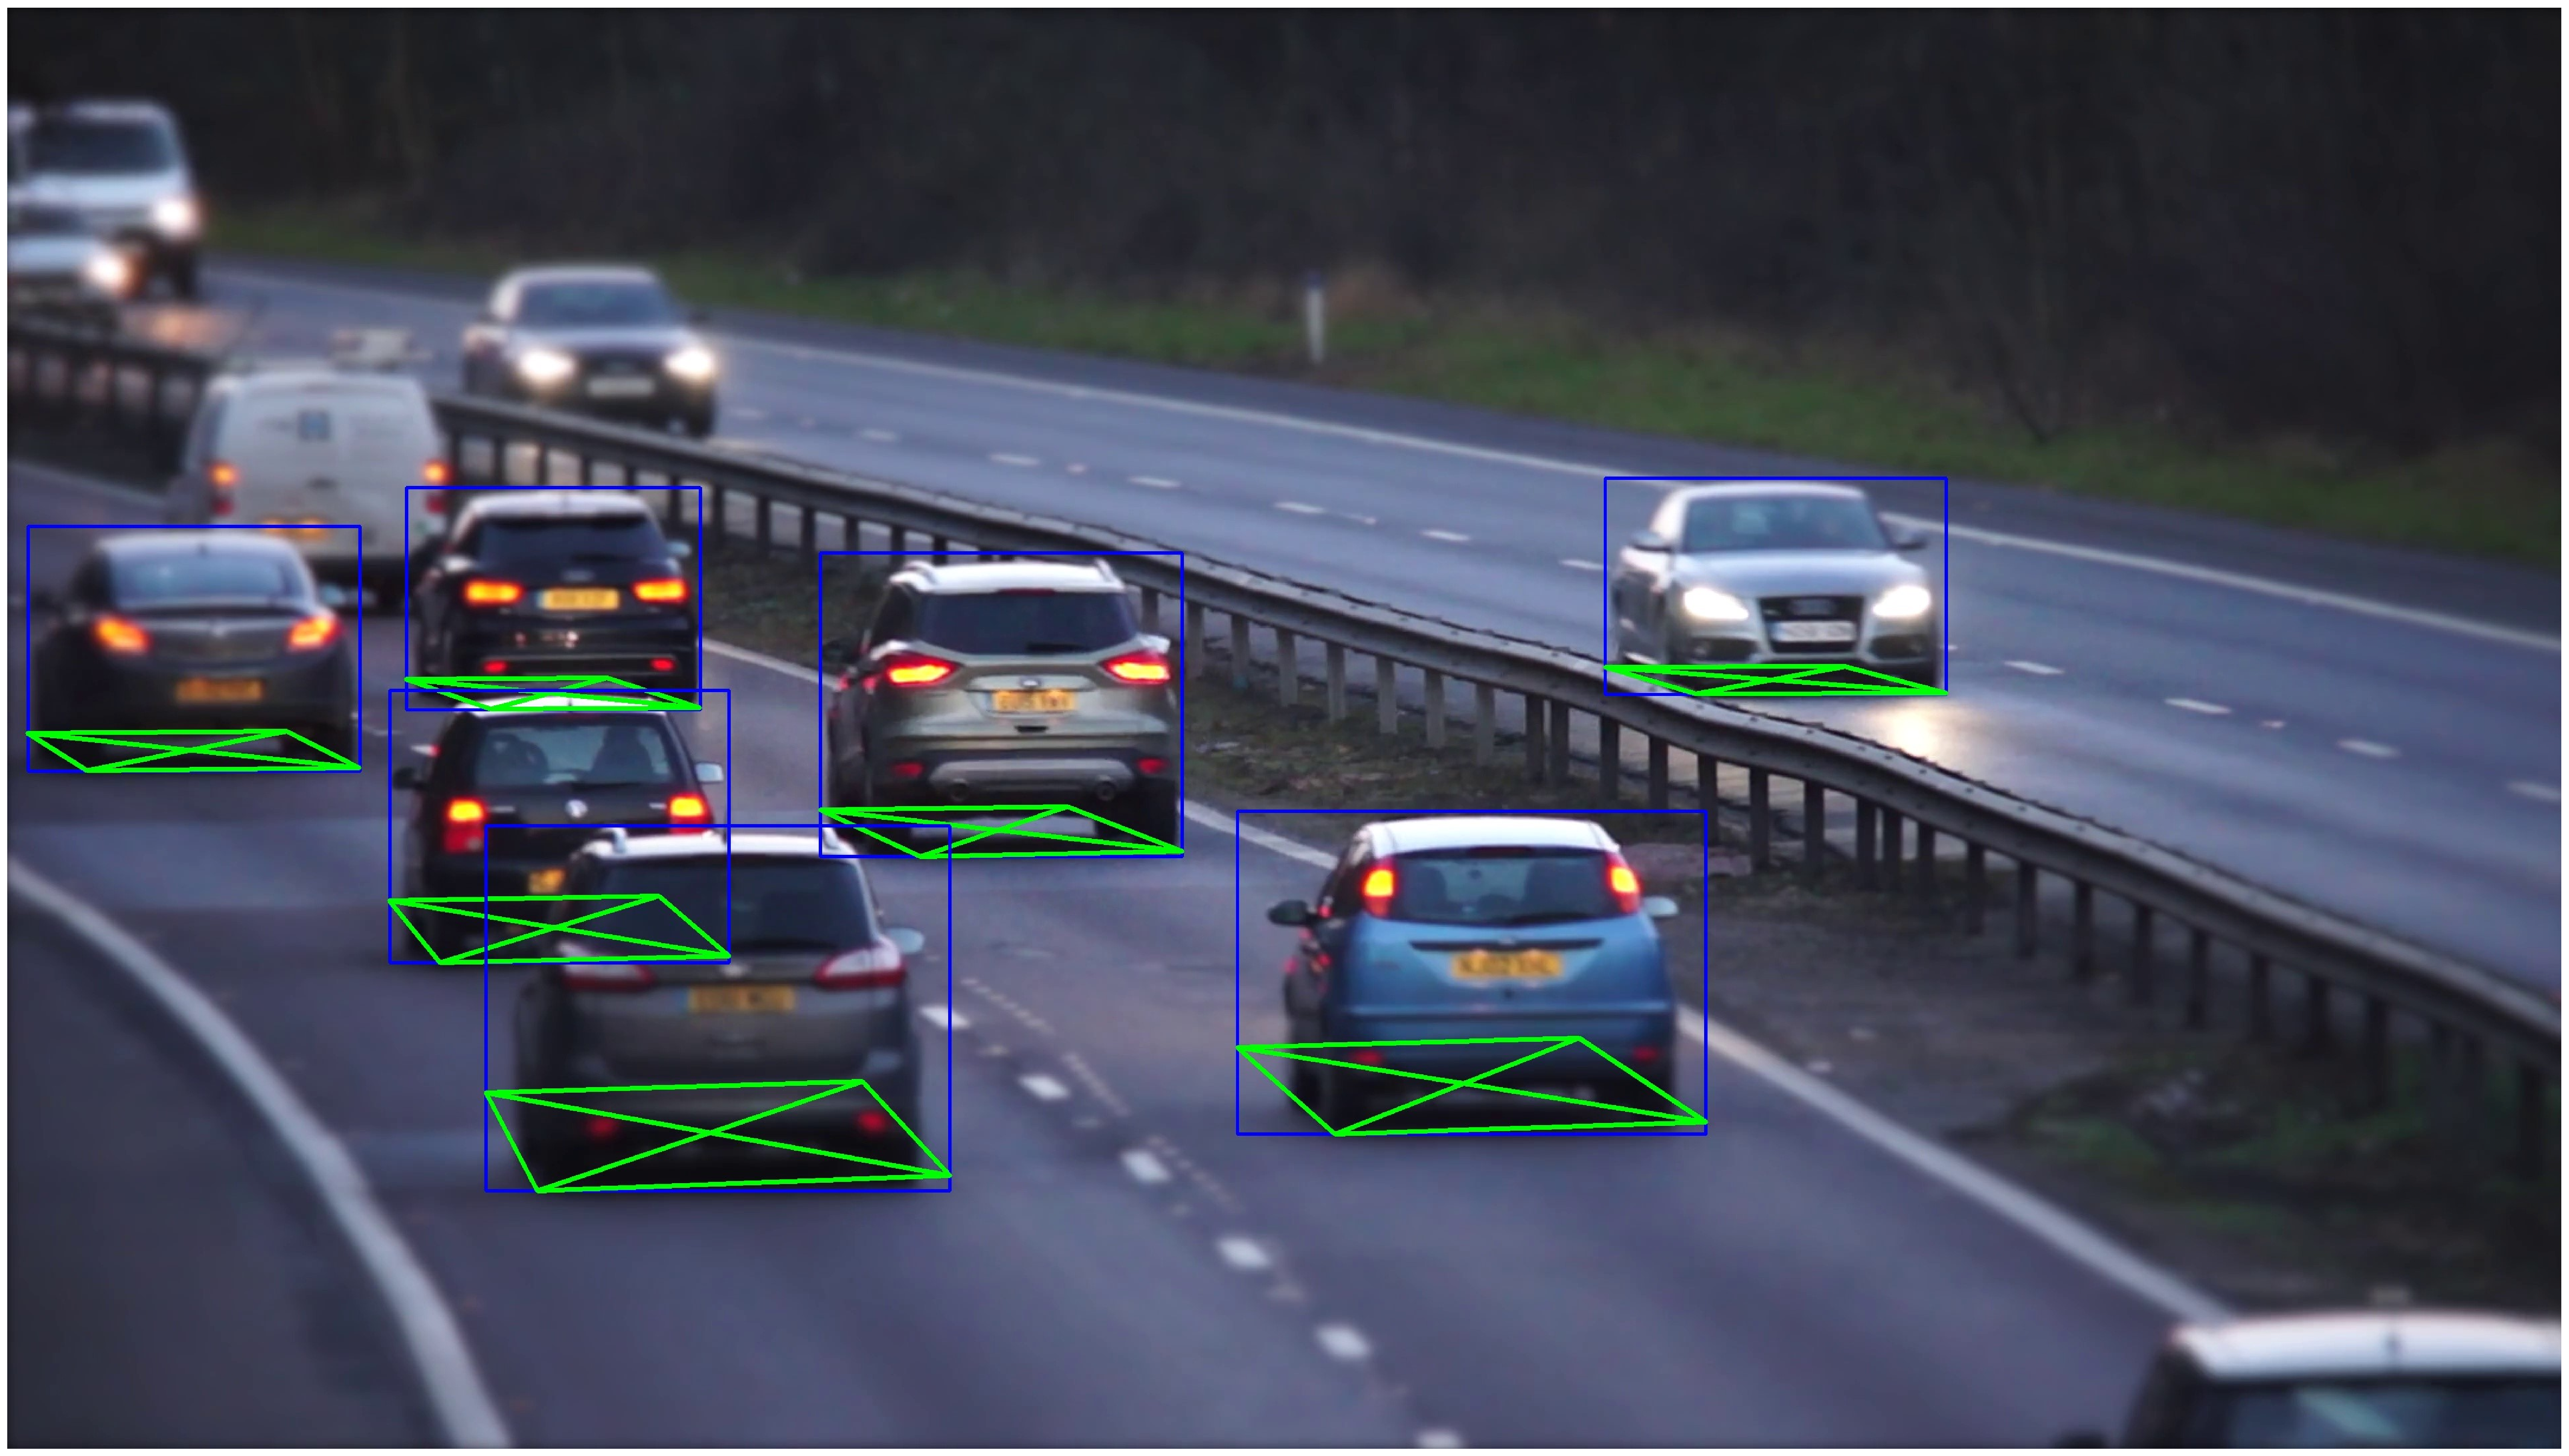
\includegraphics[height=2in]{3d_example.eps}
    \caption{2D YOLO detection with bottom projection estimation}
    \label{fig:3d_ex}
\end{subfigure}
%\hfill
\begin{subfigure}{0.19\textwidth}
\raggedleft
    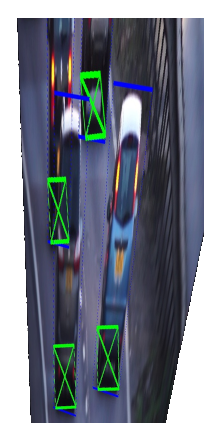
\includegraphics[height=2in]{crop_bev.eps}
    \caption{Related IPM image}
    \label{fig:bev_ex}
    \hfill
\end{subfigure}
\hfill
\caption{The visualization result of the proposed 3D object detection method}
\label{fig:met_ex}
\end{figure}


%\end{comment}

The geometric 3d reconstruction depends entirely on the 2D detector, if the vehicle model and its 2D bounding box are detected with an error, this will impact 3D detection. Nevertheless, experimental results show that the proposed approach can provide faster and more accurate 3D object localization than the state-of-art methods.

\section{Conclusion}
In this paper, a novel monocular 3D object detection framework is introduced.
Using the proposed bottom box projection reconstruction method on top of 2D tracking allows to 
improve the accuracy and performance of the 3D object detection. Moreover, the proposed
method also is highly adaptable, that allows it to be applied on top of any 2D detection and tracking algorithms.
The prospects of future research on non-static case with a moving camera will be considered.



\section{Declarations}
\begin{itemize}
    \item The author did not receive support from any organization for the submitted work.
 \item No funding was received to assist with the preparation of this manuscript.
 \item No funding was received for conducting this study.
 \item No funds, grants, or other support was received. 
 \item  The author have no relevant financial or non-financial interests to disclose.
 \item The author have no competing interests to declare that are relevant to the content of this article.
 \item All author certify that they have no affiliations with or involvement in any organization or entity with any financial interest or non-financial interest in the subject matter or materials discussed in this manuscript.
 \item The author have no financial or proprietary interests in any material discussed in this article.
 \item GitHub \url{https://github.com/DmitriyZhuravlev/3D-Object-Tracking} 
\end{itemize}


%%%%%%%%%%%%%%%%%%%%%%%% referenc.tex %%%%%%%%%%%%%%%%%%%%%
% sample references
% 
% Use this file as a template for your own input.
%
%%%%%%%%%%%%%%%%%%%%%%%% Springer%%%%%%%%%%%%%%%%%%%%%%%%%%
%
% BibTeX users please use
% \bibliographystyle{}
% \bibliography{}
%

\begin{thebibliography}{99.}%
% and use \bibitem to create references.
%
% Use the following syntax and markup for your references if 
% the subject of your book is from the field 
% "Mathematics, Physics, Statistics, Computer Science"
%
% Contribution 

\bibitem{lidar}
Shi S., Wang X., Li H.:
PointRCNN: 3D Object Proposal Generation and Detection From Point Cloud.
2019 IEEE/CVF Conference on Computer Vision and Pattern Recognition (CVPR), 2019, pp. 770-779, doi: 10.1109/CVPR.2019.00086.

\bibitem{3d_cam}
Wang Y., Zell A.:
Yolo+FPN: 2D and 3D Fused Object Detection With an RGB-D Camera.
2020 25th International Conference on Pattern Recognition (ICPR), 2021, pp. 4657-4664, doi: 10.1109/ICPR48806.2021.9413066.

\bibitem{yolo_paper}
Redmon J., Farhadi A.:
Yolov3: An incremental improvement.
arXiv preprint arXiv:1804.02767, 2018

\bibitem{traffic}
Fedorov A., Nikolskaia K., Ivanov S., Shepelev V., Minbaleev A.:
Traffic flow estimation with data from a video surveillance camera.
Journal of Big Data, vol. 6, no. 1, pp. 1–15, 2019.

\bibitem{3d_geom}
Mousavian A., Anguelov D., Flynn J., Košecká J.:
3D Bounding Box Estimation Using Deep Learning and Geometry.
2017 IEEE Conference on Computer Vision and Pattern Recognition (CVPR), 2017, pp. 5632-5640, doi: 10.1109/CVPR.2017.597.

\bibitem{lift}
Zhuravlev, D.: Lifting 2D Object Detection to 3D: Geometric Approach in Bird-Eye-View. In: Silhavy, R. (eds) Artificial Intelligence Trends in Systems. CSOC 2022. Lecture Notes in Networks and Systems, vol 502. Springer.

\bibitem{segm_trajec}
Brox T., Malik J. : Object segmentation by long-term analysis of
point trajectories. In Computer Vision–ECCV 2010, Springer, 2010, pp.
282–295.
\bibitem{segm_tracing}
Fragkiadaki K., Zhang G., Shi J. : Video segmentation by tracing
discontinuities in a trajectory embedding. In Proc. IEEE Conf. Comput. Vis. Pattern Recognit., 2012, pp. 1846–1853.

\bibitem{segm_key}
Lee Y, Kim J., Grauman K. : Key-segments for video object
segmentation. In Proc. IEEE Int. Conf. Comput. Vis., 2011, pp. 1995–
2002.
\bibitem{segm_graph}
Khoreva A., Galasso F., Hein M., Schiele B. : Classifier based graph
construction for video segmentation. In Proc. IEEE Conf. Comput. Vis.
Pattern Recognit., 2015, pp. 951–960.

\bibitem{segm_chain}
Banica D, Agape A., Ion A., Sminchisescu C. :Video object
segmentation by salient segment chain composition. In Computer
Vision Workshops (ICCVW), 2013 IEEE International Conference on,
2013, pp. 283–290.

\bibitem{segm_visual}
Papazoglou A., Ferrari V. : Fast object segmentation in
unconstrained video. Inn Computer Vision (ICCV), 2013 IEEE
International Conference on, 2013, pp. 1777–1784.

\bibitem{segm_clust}
Bandara A., Ranathunga L, Abdullah N. : Visual Feature
Clustering Using Temporal, Color and Spatial Information.
In Electronics, Communications and Networks IV (pp.677–681).

\bibitem{segm_prim}
Jang W, Lee C., Kim C. : Primary object segmentation in
videos via alternate convex optimization of foreground and background
distributions. In Proc. IEEE Conf. Comput. Vis. Pattern Recognit., 2016,
pp. 696–704.

\bibitem{segm_fusion}
Jain S., Xiong B., Grauman K. : Fusionseg: Learning to combine
motion and appearance for fully automatic segmention of generic objects
in videos. In Proc. IEEE Conf. Comput. Vis. Pattern Recognit., 2017,
pp. 3664–3673.

\bibitem{3d_geom_reduced}
Fang, J., Zhou, L., and Liu, G.:
3d bounding box estimation for autonomous vehicles by cascaded geometric constraints and depurated 2d detections using 3d results.
arXiv preprint arXiv:1909.01867, 2019.

\bibitem{bev_1}
Zhu M., Zhang S., Zhong Y., Lu P., Peng H., Lenneman J.:
Monocular 3D Vehicle Detection Using Uncalibrated Traffic Cameras through Homography.
2021 IEEE/RSJ International Conference on Intelligent Robots and Systems (IROS), 2021, pp. 3814-3821, doi: 10.1109/IROS51168.2021.9636384.

\bibitem{bev_2}
Kim Y., Kum D.:
Deep Learning based Vehicle Position and Orientation Estimation via Inverse Perspective Mapping Image.
2019 IEEE Intelligent Vehicles Symposium (IV), 2019, pp. 317-323, doi: 10.1109/IVS.2019.8814050.

\bibitem{bev_mod}
Rashed H., Essam M., Mohamed, Ei Sallab A., Yogamani S.:
BEV-MODNet: Monocular Camera based Bird's Eye View Moving Object Detection for Autonomous Driving.
2021 IEEE International Intelligent Transportation Systems Conference (ITSC), 2021, pp. 1503-1508, doi: 10.1109/ITSC48978.2021.9564667.

\bibitem{horn}
 Kanawathi J, Mokri S., Ibrahim N., Hussain A., Mustafa M.: Motion detection using Horn Schunck algorithm and implementation. 2009 International Conference on Electrical Engineering and Informatics, Bangi, Malaysia, 2009, pp. 83-87, doi: 10.1109/ICEEI.2009.5254812.

\bibitem{kmeans}
Lloyd, Stuart P.: Least squares quantization in PCM. Information Theory, IEEE Transactions on 28.2 (1982): 129-137.

\bibitem{segment}
Hafiz, A.M., Bhat, G.M.: A survey on instance segmentation: state of the art. Int J Multimed Info Retr 9, 171–
189 (2020). https://doi.org/10.1007/s13735-020-00195-x

\bibitem{fusionseg}
Jain S, Xiong B., Grauman K: Fusionseg: Learning to combine motion and appearance for fully automatic segmentation of generic objects in videos. IEEE Conference on Computer Vision and Pattern Recognition, 2017, pp. 2117–2126.



\bibitem{Hartley and Zisserman}
Hartley R., Zisserman A.:
Multiple view geometry in computer vision.
Cambridge university press, 2003

\bibitem{hom_single}
Zhou J., Li B.:
Homography-based ground detection for a mobile robot platform using a single camera.
Proceedings 2006 IEEE International Conference on Robotics and Automation, 2006. ICRA 2006., 2006, pp. 4100-4105, doi: 10.1109/ROBOT.2006.1642332.

\bibitem{adaptive_ipm} 
Jeong J., Kim A.:
Adaptive Inverse Perspective Mapping for lane map generation with SLAM.
2016 13th International Conference on Ubiquitous Robots and Ambient Intelligence (URAI), 2016, pp. 38-41, doi: 10.1109/URAI.2016.7734016.

\begin{comment}


\bibitem{kalman_mot}
Sharon M., Latha A.:
Multi-Object Tracking Based on Kalman Filter by Using Multi-Feature Appearance Model.
2018 International Conference on Inventive Research in Computing Applications (ICIRCA), 2018, pp. 544-549, doi: 10.1109/ICIRCA.2018.8597365.

\bibitem{model_det}
Ghoreyshi A., AkhavanPour A., Bossaghzadeh A.:
Simultaneous Vehicle Detection and Classification Model based on Deep YOLO Networks.
2020 International Conference on Machine Vision and Image Processing (MVIP), 2020, pp. 1-6, doi: 10.1109/MVIP49855.2020.9116922.


\bibitem{3d_mul}
Mauri A., Khemmar R., Decoux B., Haddad M., Boutteau R.:
Real-Time 3D Multi-Object Detection and Localization Based on Deep Learning for Road and Railway Smart Mobility.
J. Imaging 2021, 7, 145. https://doi.org/10.3390/jimaging7080145
\end{comment}

%
\end{thebibliography}

\end{document}
